\newpage
\section{Nah- und Fernfeld}\label{sec:NahundFern}
Antennen sind Wellenwandler, da sie die ihnen zugeführten elektromagnetischen Wellen in elektromagnetische Energie umwandeln. Diese hat ebenfalls Wellencharakter und breitet sich im Raum um die Antenne kugelförmig aus. Die zuführenden elektromagnetischen Wellen sind oft an einen elektrischen Leiter gebunden. Dies kann in Form einer Zweidrahtleitung, einer Leiterbahn auf einer Leiterplatte oder einem Koaxialkabel erfolgen. Für einige Antennen wird ein Hohlleiter als Zuleitung verwendet. 
Der Antenne kommt die Aufgabe zu, die im Leiter geführte Welle in eine Raumwelle umzuwandeln. Das bedeutet, die leitergebundene Welle wird zu einer Freiraumwelle, welche den Raum um die Antenne ausfüllt.
Hierbei passt die Antenne den Leitungswiderstand $Z_{L}$ an den Feldwellenwiderstand $Z_{F0}$ von $120\pi = 377 \ \Omega$ an. Vereinfacht kann der Wellenwiderstand im freien Raum als Wellenwiderstand im Vakuum betrachtet werden, wenn die Luft als homogenes Medium ohne Fremdkörper und demzufolge ohne Reflexionen betrachtet wird:
\begin{equation}\label{eq:Wellenimpedanz}
Z_{F0}=\sqrt{\dfrac{\mu}{\epsilon}}=\sqrt{\dfrac{\mu_{0}}{\epsilon_{0}}}=120\pi
\end{equation}
Breitet sich die Welle in einem Medium mit einer endlichen Leitfähigkeit aus, so ist die Wellenimpedanz eine komplexe Grösse, da die Leitfähigkeit des Mediums $\sigma$ berücksichtigt werden muss:
\begin{equation}\label{eq:Wellenimpedanz_Leitung}
Z_{F}=\sqrt{\dfrac{j\omega\mu_{0}}{\sigma+j\omega\epsilon}}
\end{equation}
Die Wahl der Antenne als Wellenwandlertyp hängt im wesentlichen vom gewünschten Frequenzbereich und der geforderten Antennencharakteristik ab. Bei einer Freiraumübertagungsstrecke ist die Distanz $r$ zwischen der Sende- und Empfangsantenne sehr gross verglichen mit den Abmessungen der Antennen oder der Freiraumwellenlänge $\lambda_{0}$. Vom Empfangsort scheint daher die Antennenstrahlung aus einer punktförmigen Quelle zu stammen. Dieser Entstehungspunkt der elektromagnetischen Welle wird Phasenzentrum genannt. Er ist die Quelle der abgestrahlten elektromagnetischen Felder. Die elektromagnetische Leistungsdichte, welche auf eine Empfangsantenne trifft, wird als Poynting Vektor $S$ bezeichnet.\\
 Wenn diese Voraussetzungen erfüllt sind, befindet sich der Empfangsort in der Fernfeldregion der Sendeantenne. Diese wird kurz als Fernfeld bezeichnet. Streng genommen liegen nur für Distanzen von $r\rightarrow\infty$ Fernfeldbedingungen vor. In diesem Fall können die sphärischen Phasenfronten punktweise als eben betrachtet werden. Die am Empfangsort einfallende Welle ist daher eine ebene Welle. Für die elektrischen und magnetischen Feldstärken gilt die folgende Beziehung \cite{meinke1992taschenbuch}:
\begin{equation}
E/H=120\pi\label{eq:WellenimpedanuE/H}
\end{equation}
Die Leistungsdichte $S$ ergibt sich, wenn die Feldkomponenten $E$ und $H$ senkrecht aufeinander stehen, gleichphasig sind und dieselbe Amplitude haben. Die Feldkomponenten $E$ und $H$ in (\ref{eq:LeistungsdichteS}) sind Vektoren. 
\begin{equation}
S=\dfrac{1}{2}EH=\dfrac{1}{2} E^{2}/F_{F0}\label{eq:LeistungsdichteS}
\end{equation}
Näherungsweise treten die Gesetzmässigkeiten des Fernfeldes bereits bei einem endlichen Abstand $r$ von der Sendeantenne auf. Als Grenzwert für den Fernfeldabstand ist $r_{2}$ definiert, er beschreibt den Beginn der Fernfeldregion. Für Antennen mit einer geometrischen Abmessung $D_{0}$ gilt näherungsweise\cite{meinke1992taschenbuch}:
\begin{equation}
r_{2}=\dfrac{2D_{0}^{2}}{\lambda_{0}} \label{eq:Fernfelddistanz_r2}
\end{equation}
Als $D_{0}$ ist die maximale Antennenabmessung definiert. Für Antennen mit $D_{0}=\lambda_{0}/2$ wird am Empfangsort das Phasenkriterium im Fernfeld eingehalten, da der Phasenfehler, welcher durch die Distanz der Übertragungsstrecke und die Grösse der Empfangsantenne entsteht, nicht grösser als $\lambda_{0}/8$ ist. Für den Weglängenunterschied $\Delta r$ zwischen zwei am Empfangsort einfallenden Wellen, von welchen eine am Antennenmittelpunkt und die andere am Antennenrand auftrifft, gilt gemäss (\ref{eq:Phasenfehler})\cite{meinke1992taschenbuch}:
\begin{equation}
\Delta r\leqq\lambda_{0}/8 \label{eq:Phasenfehler}
\end{equation}
Das Gebiet zwischen der Sende- und Empfangsantenne kann in Abhängigkeit von der Distanz $r$ zwischen den Antennen in drei Regionen unterteilt werden. Hierbei können keine klaren Grenzen gezogen werden, die Übergänge sind fliessend. Zwischen der Sendeantenne und der Fernfeldregion liegt die Nahfeldregion. Diese wird folgend Nahfeld genannt. Das Nahfeld wiederum kann in zwei Gebiete unterteilt werden. Es sind dies das Nahfeld und das strahlende Nahfeld. In der Nahfeldregion, welche unmittelbar die Antenne umschliesst, dominieren die reaktiven Feldkomponenten. Diese fallen mit $r^{3}$ und $r^{2}$ ab. Je nach Literatur ist die Grenze zwischen Nahfeld und strahlendem Nahfeld anders definiert. Nach dem Taschenbuch der Hochfrequenztechnik ist dieser Übergang beim Abstand $r_{1}$ erreicht, wenn $r_{1}$ der Formel (\ref{eq:Fernfelddistanz_kurzeAntenne}) entspricht\cite{meinke1992taschenbuch}.

\begin{equation}
r_{1}=0.62\sqrt{\dfrac{D_{0}^{3}}{\lambda_{0}}} \label{eq:Fernfelddistanz_kurzeAntenne}
\end{equation}
Die Bedingungen für die Nahfeldregion sind von den maximalen Antennenabmessungen abhängig. Die Definition in (\ref{eq:Fernfelddistanz_kurzeAntenne}) gilt nur für Antennen, welche als maximale Abmessung $D_{0}>\lambda_{0}$ gilt.
Bei Dipolantennen und Loop Antennen mit Abmessungen wesentlich kleiner als eine Wellenlänge $\lambda_{0}$ erstreckt sich das Nahfeld bis zum Abstand $r_{1}=\lambda_{0}/2pi$ von der Quelle. Bei einer Freiraumübertragungsstrecke, bei welcher sich die Empfangsantenne im Fernfeld der Sendeantenne im Abstand $r$ befindet, erhält man für die Leistungsdichte am Ort der Empfangsantenne \cite{meinke1992taschenbuch}:

\begin{equation}
S=\dfrac{P_{t}D}{4r^{2}\pi} = \dfrac{P_{t0}G}{4r^{2}\pi}=\dfrac{P_{ei}}{4r^{2}\pi}\label{eq:LeistungsdichteS_vonD}
\end{equation}
In (\ref{eq:LeistungsdichteS_vonD}) fällt der Faktor $4r^{2}\pi$ auf. Er kommt daher, dass die Leistungsdichte der abgestrahlten Leistung auf einer Kugeloberfläche entspricht. Der Vektor $S$ wird mit wachsendem Abstand r kleiner und besitzt die SI Einheit $[W/m^{2}]$. Für (\ref {eq:LeistungsdichteS_vonD}) gelten:
\begin{enumerate}[leftmargin=2cm]
  \item[] $P_t$: abgestrahlte Leistung [W]
  \item[] $P_{t0}$: zugeführte Leistung [W]
	\item[] $D$: Richtwert 
  \item[] $G$: Gewinn 
  \item[] $P_{ei}$: isotrope Strahlungsleistung [W] 
  \item[] $r$: Abstand zwischen Sende- und Empfangsantenne [m]
\end{enumerate} 

%Dieser Zusammenhang ist auch im Kapitel yyy in der Gleichung xxx gezeigt.




%
%\begin{figure}
%\begin{center}
%\begin{tikzpicture}
%	\draw[line width=1.5pt](2, 4) circle (0.1) node at (2,3) {Phasenzentrum};
%	\draw (2,1.5) -- (2,0);%Strich nach unten
%	\draw (2,0.3) -- (3,0.3) node at (3.5,0.5) {r};%Strich zum r
%	\draw (4,0.3) -- (5.5,0.3) ;%Strich vom r
%	
%	\draw (2.5,4) -- (3,4);
%	\draw (3.5,4) -- (4,4);
%	\draw (4.5,4) -- (5,4);
%	\draw (5.5,4) -- (6,4);
%	
%	\draw (2.5,4.05) -- (3,4.1);
%	\draw (3.5,4.15) -- (4,4.2);
%	\draw (4.5,4.25) -- (5,4.3);
%	\draw (5.5,4.35) -- (6,4.4);
%	
%	\draw (2.4,4.1) -- (2.9,4.2);
%	\draw (4.4,4.3) -- (4,3.4);
%	\draw (4.2,4.5) -- (5,4.6);
%	\draw (5.1,4.7) -- (6,3.8);
%	
%	\draw (2.5,4.2) -- (3,4.4);
%	\draw (3.5,4.5) -- (4,4.7);
%	\draw (4.5,4.8) -- (5,5);
%	\draw (5.5,5.1) -- (6,5.3);
%%	
%	\draw (2.4,3.95) -- (2.9,3.9);
%	\draw (3.4,3.85) -- (3.9,3.8);
%	\draw (4.4,3.75) -- (4.9,3.7);
%	\draw (5.4,3.65) -- (5.9,3.6);
%
%	\draw (2.3,3.9) -- (3,3.8);
%	\draw (3.3,3.7) -- (4,3.6);
%	\draw (4.3,3.5) -- (5,3.4);
%	\draw (5.3,3.3) -- (6,3.2);
%	
%	\draw (2.5,3.8) -- (3,3.6);
%	\draw (3.5,3.5) -- (4,3.3);
%	\draw (4.5,3.2) -- (5,3);
%	\draw (5.5,2.9) -- (6,2.7);
%
%%	\draw (3,3) circle (2cm);%linker Kreis
%%	\draw (7,3) circle (2cm);%rechter Kreis
%%	\draw (4.5,3) circle (0.2cm);%linker kleiner Kreis
%%	\draw (5.5,3) circle (0.2cm);%rechter kleiner Kreis
%%	\draw (4.5,3.2) -- (5.5,3.2);%Verbindung horizontal oben
%%	\draw (4.5,2.8) -- (5.5,2.8);%Verbinung horizontal unten
%%	\node[draw] at (5,6.5) {$\theta=0$};
%%	\node[draw] at (8,5.5) {$E_{\phi}(\theta)$};
%
%\end{tikzpicture}
%\end{center}
%\caption{Phasenzentrum und Pointingvektor im Antennenfeld}
%\label{fig.Phasenzentrum}
%\end{figure}
%Quelle:Taschenbuch der Hochfrequenztechnik Meineke und Grundach N2


\section{Systemansicht}
Die Systemansicht soll einen Überblick über die Bluetooth-Verbindung vom Fluginstrument zu einem Smartphone geben.
In der abschliessenden Tabelle \ref{tab:Linkbudget} werden die Annahmen und die gegebenen Parameter der Bluetooth-Verbindung aufgelistet. Mit Hilfe des Linkbudgets kann eine Abschätzung des Antennengewinns auf der Empfängerseite hergeleitet werden. Um diese Abschätzung möglich zu machen, werden einige Annahmen getroffen. Zum Beispiel geht man von einer optimalen Anpassung der Hochfrequenzquelle an die Antenne aus. Weiter wird der Luftraum zwischen Sender und Empfänger als Vakuum angenommen, was einem homogenen Ausbreitungsmedium ohne Fremdkörper entspricht.
Weitere Annahmen sind:
\begin{itemize}
\item CC2541 von TI als Sende- und Empfangschip
\item Vakuum als Ausbreitungsmedium
\item Hindernisfreie Übermittlungsstrecke
\item Energieübertragung ohne Polarisationsverluste
\item Gewinnmarge des Empfangspegels von 6 dB
\item Gewinn der Empfangsantenne von 1
\item Sendeleistung des Sendechips von 0 dBm
\item Isotrope Abstrahlung der elektromagnetischen Energie
\item Anschluss- und Verbindungsdämpfung der Antennen von 0.5 dB
\item Empfangsempfindlichkeit des CC2541 von -92 dBm bei 1 \ Mbps und 0.1\% EBR 
\end{itemize}


\subsubsection{Linkbudget}
Unter dem Linkbudget versteht man die Summe aller Leistungspegel in dB, welche vom Sender über das Übertragungsmedium bis hin zum Empfänger resultieren. Es beschreibt, welcher Signalpegel ausgehend von der Sendeleistung beim Empfänger nach Abzug aller Verluste und unter Berücksichtigung der Gewinne ankommt. Ist die Sendeleistung gesetzlich limitiert, kann die maximale Distanz der Übertragungsstrecke berechnet werden. Ist die Sendeleistung nicht beschränkt, so kann durch Umstellen der Formel die theoretisch erreichbare Sendedistanz ermittelt werden. Das Linkbudget kann nahezu beliebig komplex gestaltet werden und eine Reihe von weiteren Parametern beinhalten. In der Praxis hat sich die Berechnung des Linkbudgets bei Richtfunksystemen nach  (\ref{eq:LinkBudgetGelichung}) bewährt.

\begin{equation}
P_{Rx} = P_{Tx}+L_{Tx}+G_{x}+L_{fs}+L_{Rx}+G_{r}+L_{div}\label{eq:LinkBudgetGelichung}
\end{equation}
Die Summe (\ref{eq:LinkBudgetGelichung}) dient als Ausgangslage für die Berechnung des minimalen Gewinns der Sendeantenne $G_{x}$, welcher in dieser Arbeit den unbekannten Faktor darstellt und beim Antennendesign berücksichtigt werden muss. Da die minimale Empfängersensitivität $P_{Rx}$ aus dem Datenblatt des Bluetooth Low Energy Texas Instruments CC2541 Chip sowie die weiteren Parameter bekannt sind, kann der minimale Gewinn der Sendeantenne $G_{x}$ berechnet werden. \\

Der Empfangspegel $P_{Rx}$ aus (\ref{eq:LinkBudgetGelichung}) steht für die am Empfänger resultierende Empfangsleistung in dBm. Die Sendeleistung der Antenne wird mit $P_{Tx}$ abgekürzt und ebenfalls in der Einheit dBm angegeben. Die Übergangsverluste $L_{Tx}$ fassen jegliche Verluste durch Kabel, Verbindungen und Stecker in dB auf der Senderseite zusammen, während $L_{Rx}$ jegliche Verluste durch Kabel, Verbindungen und Stecker in dB auf Seite der Empfangsantenne bezeichnet. Der Gewinn der Sendeantenne ist als $G_{x}$ angegeben und hat die Einheit dBi. $G_{r}$ steht für den Gewinn, englisch \textit{gain}, der Empfangsantenne. $L_{fs}$ bezeichnet den Energieverlust durch die Freiraumdämpfung in der Einheit dB, $L_{div}$ steht für diverse weitere Verluste, wie zum Beispiel durch Hindernisse, oder für eine Systemreserve. \\

Die Freiraumdämpfung $L_{fs}$, englisch \textit{Free Space Path Loss}, soll an dieser Stelle genauer erläutert werden. Hierunter versteht man die Reduktion der Leistungsdichte elektromagnetischer Wellen bei der Ausbreitung im freien Raum. Anders ausgedrückt, der Pfadverlust beschreibt den Verlust an elektromagnetischer Leistung zwischen einem Sender und Empfänger. In der Theorie wird von einem isotropen Kugelstrahler ausgegangen, also einem Strahler, der gleichmässig und verlustfrei in alle Richtungen in den Raum abstrahlt. Daraus folgt, dass die abgestrahlte Energie gleichmässig in den Raum verteilt wird und somit an jedem beliebigen Punkt mit gleicher Entfernung zum Strahler identisch ist. So bilden sich Kugeln mit gleicher Leistungsdichte um den Strahler. Je grösser der Abstand zum Strahler, desto mehr verteilt sich die Energie auf eine immer grösser werdende Kugeloberfläche. Hierbei ist der Verlust durch die Freiraumdämpfung proportional zu dem Quadrat der Entfernung $R$ zwischen Sender und Empfänger und zu dem Quadrat der verwendeten Frequenz \cite{linkbudget}.
\clearpage
\newpage

%%%%%%%%%%%%%%%%%%%%%%%%%%%%%%%%%%%%%%%%%%%%%%%%%%%%%%%%%%
\begin{figure}[!ht]
\begin{center}
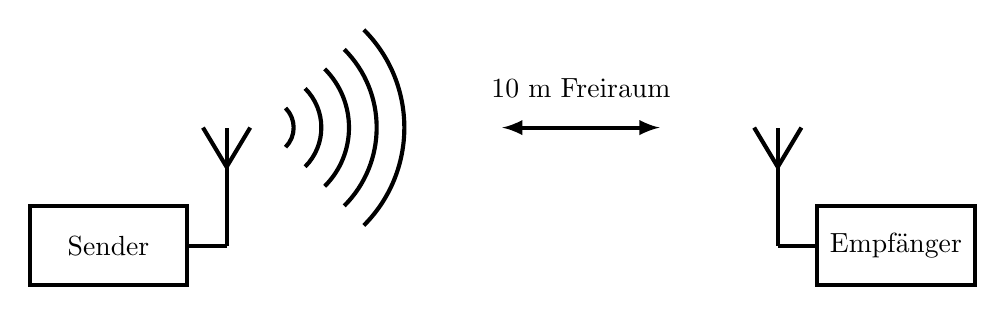
\begin{tikzpicture}
	\draw[line width=1.5pt](0, 0) rectangle (2, 1) node[pos=0.5] {Sender};
	\draw[line width=1.5pt] (2, 0.5) -- (2.5, 0.5);%zuleitung
	\draw[line width=1.5pt] (2.5, 0.5) -- (2.5, 1.5);%Antennenmast
	\draw[line width=1.5pt] (2.5, 1.5) -- (2.2, 2);%Antenne
	\draw[line width=1.5pt] (2.5, 1.5) -- (2.8, 2);
	\draw[line width=1.5pt] (2.5, 1.5) -- (2.5, 2);
	
	\draw[line width=1.5pt, <->, >=latex](6, 2) -- (8, 2) node at (7, 2.5) {10 m Freiraum};
	
	\draw[line width=1.5pt] (9.5, 0.5) -- (10, 0.5);%zuleitung
	\draw[line width=1.5pt] (9.5, 0.5) -- (9.5, 1.5);%Antennenmast
	\draw[line width=1.5pt] (9.5, 1.5) -- (9.2, 2);%Antenne
	\draw[line width=1.5pt] (9.5, 1.5) -- (9.8, 2);
	\draw[line width=1.5pt] (9.5, 1.5) -- (9.5, 2);
	\draw[line width=1.5pt,decorate,decoration=expanding waves](3, 2) -- (5, 2);
	\draw[line width=1.5pt](10, 0) rectangle (12, 1) node[pos=0.5] {Empfänger};
	%\node[draw,text] at (1,0.5) {Sender};
%	\node[draw,text] at (9,0.5) {Empfenger};
\end{tikzpicture}
\end{center}
\caption{Verbindungsmodell}
\label{fig:LinkModell}
\end{figure}
%%%%%%%%%%%%%%%%%%%%%%%%%%%%%%%%%%%%%%%%%%%%%%%%%%%%%%%%%%%

Die Abbildung \ref{fig:LinkModell} zeigt ein einfaches Verbindungsmodell eines Kommunikationskanals. Das in der Tabelle \ref{tab:Linkbudget} aufgezeigte Linkbudget listet alle in (\ref{eq:LinkBudgetGelichung}) auftretenden Parameter einer Signalübertragung auf. Es werden einige Vereinfachungen getroffen. Der Gewinn der Empfangsantenne $G_{r}$ ist mit Faktor 1 definiert, das entspricht 0 dBi. Es werden keine Polarisationsverluste berücksichtigt. Für die Berechnung der Freiraumdämpfung $L_{fs}$ wird als Übertragungsmedium Vakuum angenommen und die Übertragungsdistanz enspricht 10 Meter. Als Sende- und Empfangschip kommt der Texas Instruments CC2541 Chip zu Anwendung. Für die Berechnung der Freiraumdämpfung müssen die folgenden Definitionen und Formeln genannt weden \cite{Tekom}:
 
\begin{eqnarray}
  	d_{0} 	&=& 10 [m] \\ \label{eq:d0_LinkBudget}
  G_r		&=& 1 \\ \label{eq:Gr_LinkBudget}
	G_t 		&=& 1 \\ \label{eq:Gt_LinkBudget}
  P_{Rx}(d_0) 	&=& \dfrac{P_{Tx}G_t G_r\lambda^2}{(4\pi)^2 d_0^2} \\ \label{eq:Prx_LinkBudget}
  L_{fs} 		&=& \dfrac{P_{Tx}}{P_{Rx}} \\ \label{eq:Freiraumdaempfung}
  L_{fs}(dB) 	&=& 10\log_{10}(L_{fs}) \\ \label{eq:Freiraumdaempfung_dB}
  L_{fs}(dB) 	&=& 20\log(\dfrac{4\pi d_0 f_0}{c_0}) \label{eq:Freiraumdaempfung_dB_aufgelöst} 
\end{eqnarray}
Durch Auflösen der Gleichung (\ref{eq:Freiraumdaempfung_dB}) erhält man für eine Übertragungsstrecke von 10 Metern und einer Signalfrequenz von 2.45 GHz eine Signaldämpfung von -60dB. Man beachte das Minus in (\ref{Freiraumdämpfung_ausgerechnet}). Der erhaltene Wert muss negativ sein, da es sich um eine Dämpfung handelt.
\begin{equation}\label{Freiraumdämpfung_ausgerechnet}
  L_{fs}(dB) = -20\log(\dfrac{4\pi 10[m] 2.45*10^9 [1/s] }{3*10^8[m/s]}) =-60.2dB
\end{equation}

\begin{table}[!ht]
 \centering
 \begin{tabular}{l c r} \toprule 
 Komponete               	& 			&Leistungsbeitrag  \\ \midrule
  Abgegebene Leitung    			&$P_{Tx}$ 	& 0dB       \\
  Übergangsverluste              &$L_{Tx}$	& -3dB       \\
  Gewinn der Sendeantenne    	&$G_{x}$		& zu bestimmen        \\
  Ausbreitungsverluste   		& $F_{LS}$	& -60dB        \\
  Gewinn Empfangsantenne  		& $G_{r}$	& 0dB           \\
  Polarisationsverluste          & 	& 0dB            \\
  Übergangsverluste              & $L_{Rx}$	& -3dB            \\
  Erwartete Leistung am Empfänger & $P_{Rx}$  & -66dBm \cite{CC2541} \\ \midrule
  Systemreserve        			 & $L_{div}$&-6dBm \\ 
  Minimal notwendiges Empfängersignal &$P_{Rx}^{'}$ & -72dB \\ \bottomrule
  \end{tabular}
  \caption{Linkbudget 10m Bluetooth Übertragung}
  \label{tab:Linkbudget}
\end{table}

Tabelle \ref{tab:Linkbudget} zeigt die für die Bluetooth-Verbindung relevanten Gewinne und Verluste des Übertragungskanals. Bei einer Verbindung von 10 Metern und den getroffenen Vereinfachungen ist mit einem minimalen Empfangspegel von $-72\ dB$ am Empfänger zu rechnen. Da die minimale Empfangssensitivität bei $-92\ dB$ liegt, entspricht dies einem ausreichenden Empfangspegel, es resultiert sogar eine Reserve von $20\ dB$. Da sich, wie aus (\ref{gain}) ersichtlich wird, der Gewinn einer Antenne aus dem Richtfaktor $D$ und dem Wirkungsgrad $\eta$ zusammensetzt, kann an dieser Stelle keine konkrete Aussgage zum Gewinn der Sendeantenne $G_{Tx}$ gemacht werden, da diese beiden Parameter nicht bekannt sind. Bei einem realen Antennendesign wird der Wirkungsgrad mit Sicherheit nicht 1 betragen und das Abstrahlverhalten nicht kugelförmig sein. Keine praktisch realisierbare Antenne zeigt ein rein isotropes Verhalten, da sich unter anderem die absorbierenden Eigenschaften des  Gerätes in der Feldausbreitung bemerkbar machen. 

%%%%%%%%%%%%%%%%%%%%%%%%%%%%
%%%%Quelle&%%%%%%%%%%%
%%%%%%%%%%%%%%%%%%%%%%%%%

\section{Quelle}
Jedes Antennensystem verfügt über eine Quelle. Diese liefert an ihrem Ausgang ein hochfrequentes Signal, dessen Übertragungskanal entweder symmetrisch oder asymmetrisch sein kann. Die Ausgangsimpedanz von Quellen kann sehr unterschiedlich sein. Oft befindet sich am Quellenausgang ein Anpassungsnetzwerk, welches die Quellenimpedanz an die Leitungsimpedanz anpasst. Die in der Hochfrequenztechnik verwendeten Quellen haben oft einen Innenwiderstand von $50\ \Omega$. Die Abbildung \ref{fig:asymetrischeQuelle} zeigt eine asymmetrische  Hochfrequenzquelle. Einer der beiden Anschlüsse wird als Massenpotential definiert, der andere Anschluss führt das gewünschte Signal. Der Innenwiderstand der gezeigten Quelle ist $50\ \Omega$ reell.
\begin{figure}[!th]
	\begin{center}
	\begin{tikzpicture}
	\draw[line width=1.5pt](3, 3.5) circle (0.5) node at (3,3.5) {Uq};
	\draw[line width=1.5pt] (3, 5) -- (4.5, 5);
	%\draw[line width=1.5pt] (3, 2) -- (7, 2);
	\draw[line width=1.5pt, -*](3, 2)  -- (7, 2);
	\draw[line width=1.5pt] (3, 2) -- (3, 3);
	\draw[line width=1.5pt] (3, 4) -- (3, 5);
	\draw[line width=1.5pt](4.5, 4.75) rectangle (5.5, 5.25) node at (5, 5.5) {Rq} node at (5, 4.5) {50 Ohm};
	%\draw[line width=1.5pt] (5.5, 5) -- (7, 5);
	\draw[line width=1.5pt, -*](5.5, 5)  -- (7, 5);
	\draw[line width=1.5pt, decorate, decoration=snake](8, 5) -- (9, 5) node at (8.5, 5.5) {Signal der Quelle};
	\draw[line width=1.5pt](2, 1.5) rectangle (6.5, 6) ;%Quellenramen
	\draw[line width=1.5pt] (7, 2) -- (8, 2);%Masse Strich horizontal
	\draw[line width=1.5pt] (8, 2) -- (8, 1.5);%Masse Strich vertikal
	\draw[line width=1pt] (7.5, 1.5) -- (8.5, 1.5);%Masse Strich horizontal kurz
	\draw[line width=1pt] (7.7, 1.3) -- (8.3, 1.3);%Masse Strich horizontal kurz
	\draw[line width=1pt] (7.9, 1.1) -- (8.1, 1.1);%Masse Strich horizontal kurz
	\end{tikzpicture}
	\end{center}
\caption{Ersatzschaltbild einer asymmetrischen Quelle}
\label{fig:asymmetrischeQuelle}
\end{figure}
Bei asymmetrischer Signalübertragung erfolgt diese in Form einer Spannung, welche sich gegenüber einem Bezugspotential ändert. Dies ist die einfachste Art der Datenübertragung. Das Bezugspotential wird auf einer Referenzleitung übertragen, es entspricht meistens dem Massenpotential. \\

Symmetrische Quellen haben drei Anschlusspunkte. Das Hochfrequenzsignal wird auf zwei Leitungen übertragen. Die Signalform ist auf den beiden Leitungen um 180$^\circ$  zueinander verschoben. Eine symmetrische Quelle ist in Abbildung \ref{fig:symmetrischeQuelle} dargestellt.

\begin{figure}[!ht]
	\begin{center}
	\begin{tikzpicture}
	\draw[line width=1.5pt](3, 3.5) circle (0.5) node at (3,3.5) {Uq};
	\draw[line width=1.5pt] (3, 5) -- (4.5, 5);
	%\draw[line width=1.5pt] (3, 2) -- (7, 2);
	\draw[line width=1.5pt, -*](3, 2)  -- (8, 2);
	\draw[line width=1.5pt] (3, 2) -- (3, 3);
	\draw[line width=1.5pt] (3, 4) -- (3, 5);
	%\draw[line width=1.5pt](4.5, 4.75) rectangle (5.5, 5.25) node at (5, 5.5) {Rq} node at (5, 4.5) {50 Ohm};
	\draw[line width=1.5pt] (4.5, 4) -- (4.5, 6);%Spliter
	\draw[line width=1.5pt] (4.5, 6) -- (5.5, 6);%Spliter oben
	\draw[line width=1.5pt] (4.5, 4) -- (5.5, 4);%Spliter unten
	\draw[line width=1.5pt] (5.5, 5.5) -- (5.5, 6.5);%Verstärker hinten
	\draw[line width=1.5pt] (5.5, 6.5) -- (6.5, 6);%obenaben
	\draw[line width=1.5pt] (5.5, 5.5) -- (6.5, 6);%untenufen
	\draw[line width=1.5pt] (5.5, 3.5) -- (5.5, 4.5);%Inverter hinten
	\draw[line width=1.5pt] (5.5, 4.5) -- (6.5, 4);%obenaben
	\draw[line width=1.5pt] (5.5, 3.5) -- (6.5, 4);%untenufen
	\draw[line width=1.5pt, -*](6.5, 6)  -- (8, 6);%Siganlpfad oben
	\draw[line width=1.5pt](6.6, 4) circle (0.1);
	\draw[line width=1.5pt, -*](6.7, 4)  -- (8, 4);%Siganlpfad unten
	\draw[line width=1.5pt, decorate, decoration=snake](9, 6) -- (10, 6) node at (9.5, 6.5) {Signal der Quelle};
	\draw[line width=1.5pt, decorate, decoration=snake](9, 4) -- (10, 4) node at (9.5, 4.5) {Signal der Quelle invertiert};
	\draw[line width=1.5pt](2, 1.5) rectangle (7, 6.8) ;%Quellenramen
	\draw[line width=1.5pt] (8, 2) -- (9, 2);%Masse Strich horizontal
	\draw[line width=1.5pt] (9, 2) -- (9, 1.5);%Masse Strich vertikal
	\draw[line width=1pt] (8.5, 1.5) -- (9.5, 1.5);%Masse Strich horizontal kurz
	\draw[line width=1pt] (8.7, 1.3) -- (9.3, 1.3);%Masse Strich horizontal kurz
	\draw[line width=1pt] (8.9, 1.1) -- (9.1, 1.1);%Masse Strich horizontal kurz
	\end{tikzpicture}
	\end{center}
\caption{Ersatzschaltbild einer symmetrischen Quelle}
\label{fig:symmetrischeQuelle}
\end{figure}
\newpage
\section{Zuleitung}
Hierunter versteht man die Verbindung zwischen Quelle und Antenne. Je nach System kommt eine Zweidrahtleitung oder eine Koaxialleitung zum Einsatz. Eine Zweidrahtleitung ist eine symmetrische Verbindung, während ein Koaxialkabel eine asymmetrische Verbindung darstellt.
Weitere Verbindungstypen sind:
\begin{itemize}
\item Hohlleiter
\item Glasfaserleiter
\end{itemize}
An dieser Stelle soll genauer auf die elektrische, leitergebundene Übertragung eingegangen werden.
Leitungen gehören zu den wichtigsten Übertragungsmedien der Nachrichtentechnik. Sie übertragen elektromagnetische Wellen fast mit Lichtgeschwindigkeit vom Sende- zum Empfangsort. Bei Gleichstrom und sehr niedrigen Frequenzen kann eine Leitung im Allgemeinen als ideal bezeichnet oder mit einem rein ohmschen Verhalten angenommen werden. Somit können die Signalverläufe am Eingang und Ausgang näherungsweise als identisch und zeitgleich bezeichnet werden. Kommt aber die physikalische Länge der Leitung in die Grössenordnung der Wellenlänge der zu übertragenden Schwingung oder die Anstiegszeit eines Impulses in die Grössenordnung der Ausbreitungsverzögerung, dann kann die Ausgangsspannung völlig anders aussehen als die Eingangsspannung. Die Leitung muss jetzt als Zweitor mit frequenzabhängigen Eigenschaften betrachtet werden.
Ein geeignetes Konzept für die Betrachtung und das  Verständnis eines frequenzabhängigen Zweitors bringt der Begriff der elektrischen Länge mit sich:
\begin{equation}
Elektrische \  L\"ange=\dfrac{l}{\lambda}\label{eq:ElektrischeLänge}
\end{equation}

In (\ref{eq:ElektrischeLänge}) entspricht $l$ der Länge der Leitung und $\lambda$ der Wellenlänge des Signales auf der Leitung. Zur Analyse, ob eine Leitung strahlt, wird ihre $elektrische \  Länge$ betrachtet. Bei einer $elektrischen  \ L\"ange\ \dfrac{l}{\lambda} \le \dfrac{1}{20}$  kann die Leitung mit der klassischen Schaltungstheorie behandelt und als verlustlos und reflexionsfrei betrachtet werden. Ein anderes Bild zeigt sich bei einer $elektrischen \ L\"ange\ \dfrac{l}{\lambda}>\dfrac{1}{20}$. In diesem Fall muss die Leitung als frequenzabhängiges Zweitor betrachtet werden. Die Phänomene der elektromagnetischen Wellen werden wirksam, die Leitungen müssen mit ihren frequenzabhängigen Eigenschaften behandelt werden. \\

Geht man von einer idealen Wellenausbreitung aus, bei der keine Verluste vorkommen, so ist die Wellenlänge $\lambda$ mit der Signalfrequenz $f$ und der Lichtgeschwindigkeit $c_0$ wie gemäss (\ref{eq:WellenlängeMITc}) verknüpft \cite{Tekom}:
\begin{equation}
\lambda_{0}=\dfrac{c}{f}\label{eq:WellenlängeMITc}
\end{equation}
Da eine Leitung immer verlustbehaftet ist, kann die Ausbreitung einer Welle im Leitermedium nie der Lichtgeschwindigkeit $c_0$ entsprechen. Daher gilt:
\begin{equation}
\lambda=\dfrac{v}{f}\label{eq:WellenlängeMITv}
\end{equation}
Die Signalgeschwindigkeit $v$ dividiert durch die Frequenz ergibt die Wellenlänge $\lambda$. Für die Gleichungen (\ref{eq:ElektrischeLänge}), (\ref{eq:WellenlängeMITc}) und (\ref{eq:WellenlängeMITv}) gilt:
\begin{enumerate}[leftmargin=2cm]
   \item[] $l$: Leitungslänge [m] 
   \item[] $\lambda$: Wellenlänge  [m] 
   \item[] $f$: Frequenz (Hz) [1/s] 
   \item[] $c_0$: Lichtgeschwindigkeit  [m/s] 
   \item[] $v$: Geschwindigkeit  [m/s] 
\end{enumerate} 
Besonders vorteilhafte Übertragungseigenschaften hat die längshomogene Leitung. Es handelt sich dabei um eine Leitung, welche auf ihrer ganzen Länge einen konstanten Leitungsquerschnitt, gleiches
Leitermaterial, konstanten Leiterabstand und einen gleichförmigen Isolator aufweist. Gebräuchliche Formen sind die symmetrische Zweidrahtleitung, die verdrillte Zweidrahtleitung, die Streifenleitung auf einer Printplatte oder das Koaxialkabel.
\subsection{Leitungsmodell}
Um die Zweitoreigenschaften einer längshomogenen Zweidrahtleitung zu ermitteln, wird diese in $n$ identische Elementarzweitore mit einer Länge von $\Delta z$ unterteilt, wie dies in Abbildung \ref{fig:LeitungsmodellZweitorKette} dargestellt ist. Die Gesamtlänge der Leiter $l$ ergibt sich aus n$\Delta z$. Hierbei soll $n$ sehr gross sein, damit $\Delta z$ verschwindend klein wird.

\begin{figure}[!ht]
	\begin{center}
	\begin{tikzpicture}
	%unten
	\draw[line width=0.5pt, *-*](2, 2)  -- (3.5, 2);
	\draw[line width=0.5pt, -*](3.5, 2)  -- (5, 2);
	\draw[line width=0.5pt, -*](5, 2)  -- (6.5, 2) ;
	\draw[line width=0.5pt, -*](6.5, 2)  -- (8, 2);
	\draw[line width=0.5pt, -*](8, 2)  -- (9.5, 2);
	%oben
	\draw[line width=0.5pt, *-*](2, 3.5)  -- (3.5, 3.5);
	\draw[line width=0.5pt, -*](3.5, 3.5)  -- (5, 3.5);
	\draw[line width=0.5pt, -*](5, 3.5)  -- (6.5, 3.5) node at (5.75,4) {$\Delta z$};
	\draw[line width=0.5pt, -*](6.5, 3.5)  -- (8, 3.5);
	\draw[line width=0.5pt, -*](8, 3.5)  -- (9.5, 3.5)node at (7.9,4) {$n$};
	\draw[line width=1.5pt, ->, >=latex](2, 3.2) -- (2, 2.3) node at (1.5,2.75) {$\underline{U_{1}}$};
	\draw[line width=1.5pt, ->, >=latex](9.5, 3.2) -- (9.5, 2.3) node at (10,2.75) {$\underline{U_{2}}$};
	%vertikal gepunktete linien
	\draw[line width=0.5pt, style=dashed](3.4, 2) -- (3.4, 3.5);%vertikal gepunktete Linie
	\draw[line width=0.5pt, style= dashed](4.9, 2) -- (4.9, 3.5);%vertikal gepunktete Linie
	\draw[line width=0.5pt, style= dashed](6.4, 2) -- (6.4, 3.5);%vertikal gepunktete Linie
	\draw[line width=0.5pt, style=dashed](7.9, 2) -- (7.9, 3.5);%vertikal gepunktete Linie
	\end{tikzpicture}
	\end{center}
\caption{Leitungsmodell einer Zweitorkette}
\label{fig:LeitungsmodellZweitorKette}
\end{figure}
Aus der Elektrotechnik ist bekannt, dass sich beim Einschalten einer Signalquelle auf der Leitung ein Strom $i(t)$ einstellt. Die Folge davon ist ein magnetisches Feld radial um die Leitung. Der magnetische Fluss ergibt sich mit der Abschnittsinduktivität zu $\Phi = i  \Delta L$. Das Einschalten der Quelle führt weiter zu einer Spannung zwischen den Leitern, was widerum zu einem elektrischen Feld und einer Oberflächenladung $Q = u  \Delta C$ auf den Leitern führt. Diese beiden Sachverhalte sind in den Ablildungen \ref{Magnetischer Fluss einer Zweidrahtleitung}	 und \ref{fig:statischeZeidrahtleitung} dargestellt, wobei es sich um eine statische Feldbetrachtung der transversalen Ebene  einer Zweidrahtleitung handelt. \cite{Tekom}.
\begin{figure}[!h]
\begin{minipage}{7cm}
	\centering
	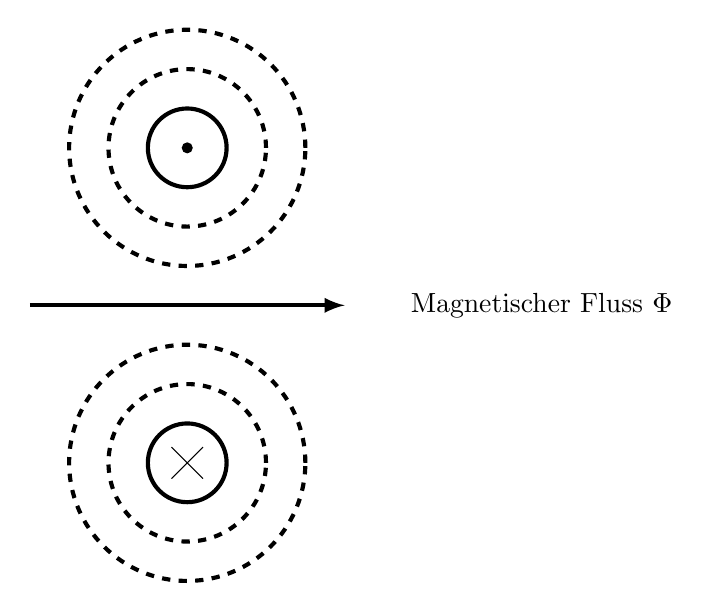
\begin{tikzpicture}
		\draw[line width=1.5pt,style=dashed](5, 1.5) circle (1.5);
		\draw[line width=1.5pt,style=dashed](5, 1.5) circle (1);
		\draw[line width=1.5pt](5, 1.5) circle (0.5);
		\draw(4.8, 1.3)  -- (5.2, 1.7);
		\draw(4.8, 1.7)  -- (5.2, 1.3);
		\draw[line width=1.5pt, ->, >=latex](3, 3.5) -- (7, 3.5) node at (9.5,3.5){Magnetischer Fluss $\Phi$};
		\draw[line width=1.5pt,style=dashed](5, 5.5) circle (1.5);
		\draw[line width=1.5pt,style=dashed](5, 5.5) circle (1);
		\draw[line width=1.5pt](5, 5.5) circle (0.5);
		\fill[fill=black](5, 5.5) circle (2pt);				
	\end{tikzpicture}
	\caption{Magnetischer Fluss einer Zweidrahtleitung}	
\end{minipage}
\hfill
\begin{minipage}{7cm}
	\centering
	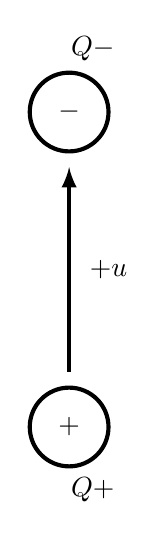
\begin{tikzpicture}
		\draw[line width=1.5pt](5, 1.5) circle (0.5) node at (5, 1.5){$+$};
		\draw node at (5.3,0.7){$Q+$};
		\draw[line width=1.5pt, ->, >=latex](5, 2.2) -- (5, 4.8) node at (5.5,3.5){$+u$};
		\draw[line width=1.5pt](5, 5.5) circle (0.5) node at (5, 5.5){$-$};
		\draw node at (5.3,6.3){$Q-$};	
	\end{tikzpicture}
	\caption{Oberflächenladung einer Zweidrahtleitung}		
%\caption{statische Feldbetrachtung einer Transversalen Ebene einer Zeidrahtleitung}
\end{minipage}
\label{fig:statischeZeidrahtleitung}

\end{figure}

\begin{figure}[!ht]
	\centering
	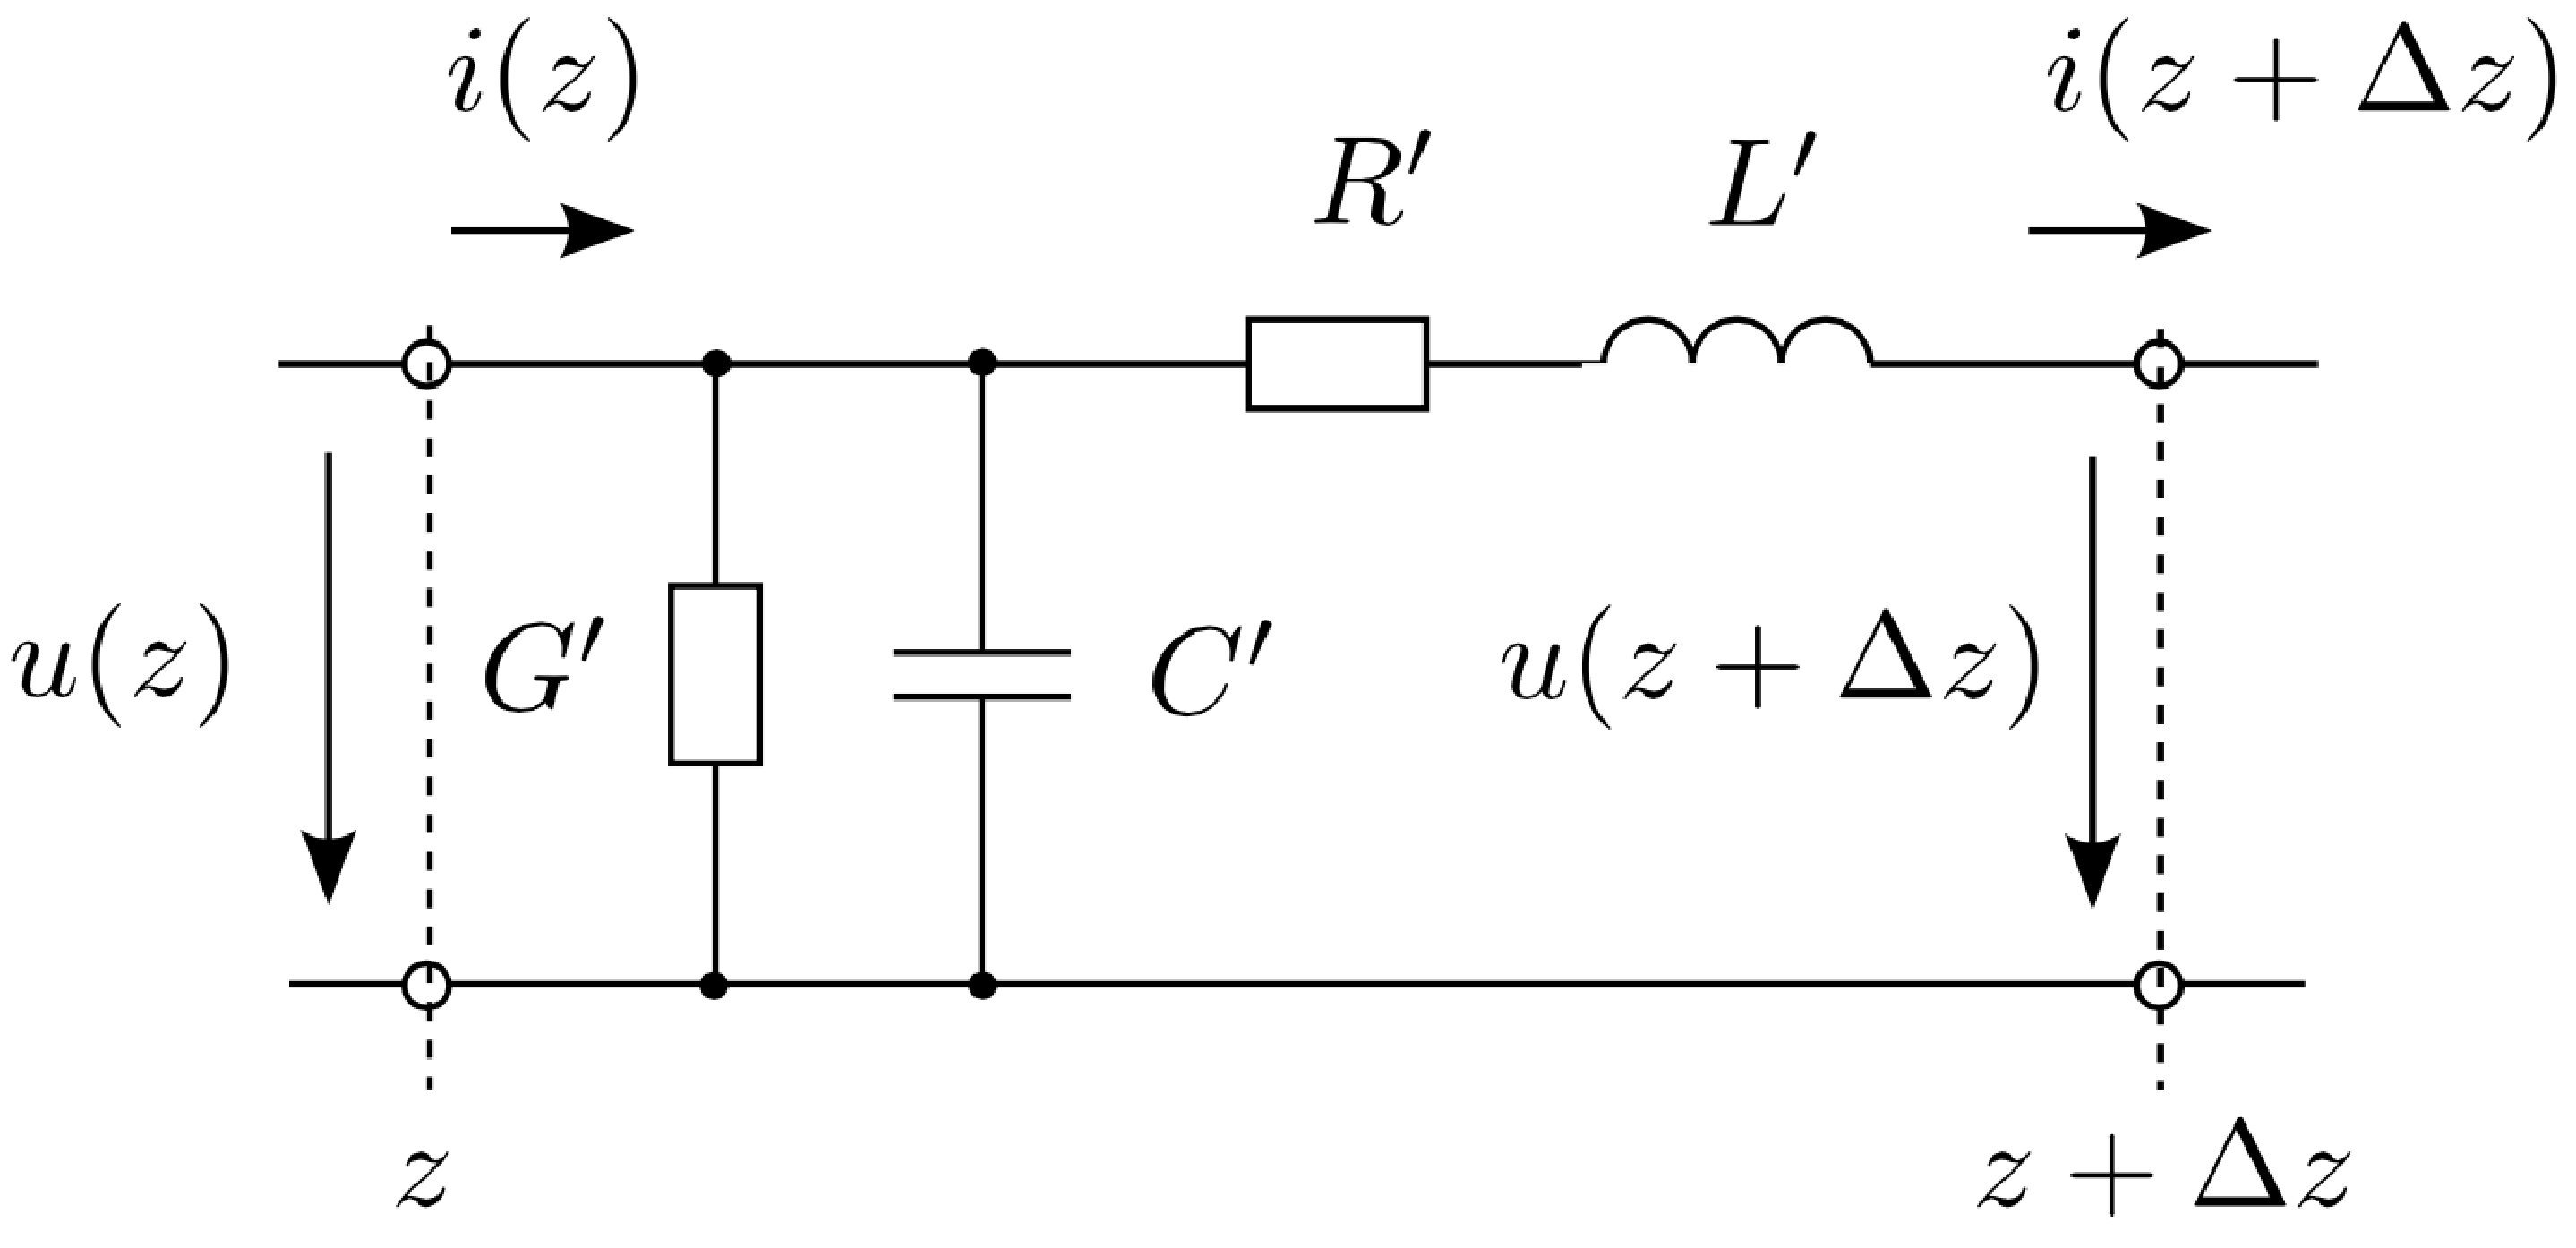
\includegraphics[width=11cm]{content/bilder/Leiterstueck.pdf}%
	\caption{Ersatzschaltbild eines elementaren Leiterstücks}
	\label{fig:ESBLeiterstueck}
\end{figure}
Bei einer längshomogenen Leitung darf die Annahme getroffen werden, dass die Induktivität $\Delta L$ und die Kapazität $\Delta C$ gleichförmig über die Länge $\Delta z$ verteilt sind. Man kann sie daher im Modell als Leitungsbeläge ausdrücken. Die Gleichung (\ref{eq:InduktiverLeitungsbelag}) gibt den Induktivitätsbelag, die Gleichung (\ref{eq:KapazitiverLeitungsbelag})  den Kapazitätsbelag wieder.

\begin{equation}
L'=\dfrac{\Delta L}{\Delta z}\label{eq:InduktiverLeitungsbelag}
\end{equation}
\begin{equation}
C'=\dfrac{\Delta C}{\Delta z}\label{eq:KapazitiverLeitungsbelag}
\end{equation}
Werden zudem die ohmschen Verluste im Leiter $R'$ und allfällige dielektrische Verluste in der Isolation $G'$ als Wirkwiderstände dargestellt, so lässt sich das Ersatzschaltbild eines Zweitores mit der Länge $\Delta z$ gemäss Abbildung \ref{fig:ESBLeiterstueck} modellieren.
Für die Abbildung \ref{fig:ESBLeiterstueck} gelten die Zusammenhänge aus den Gleichungen (\ref{eq:KapazitiverLeitungsbelag}) und  (\ref{eq:KapazitiverLeitungsbelag}) \cite{Tekom}.
\begin{enumerate}[leftmargin=2cm]
   \item[] $R'$: Widerstandsbelag [$\Omega/m$] 
   \item[] $L'$: Induktivitätsbelag  [$H/m$] 
   \item[] $G'$: Dielektrische Verluste/m  [$S/m$] 
   \item[] $C'$: Kapazitätsbelag [$F/m$] 
   \item[] $\Delta z$: Zweitorlänge [$m$] 
\end{enumerate} 
Auf einer Leitung sind immer eine vorwärts sowie  eine rückwärts laufende Strom- und Spannungswelle vorhanden, ausser die vorwärts laufende Welle wird vollständig von einer Last absorbiert. Die vorwärts laufende Welle breitete sich entlang der positiven z-Achse, die rückwärts laufende Welle entlang der negativen z-Achse aus. Spannung und Strom auf der Leitung können als Summe dieser zwei Wellen beschrieben werden. Mit Hilfe der elementaren Leiterabschnitte können sie an jedem Punkt $z$ der Leitung berechnet werden. Die Gleichung (\ref{eq:UvonZundT}) gibt die Summe der Spannungswellen, die Gleichung (\ref{eq:IvonZundT}) die Summe Stromwellen wider \cite{Tekom}.
\begin{eqnarray}\label{eq:UvonZundT}
U(z,t) &=& U_{v}e^{-\alpha z}e^{j(\omega t -\beta z)}+U_{r}e^{\alpha z}e^{j(\omega t \beta z)}
\end{eqnarray}
\begin{eqnarray}\label{eq:IvonZundT}
I(z,t) &=& I_{v}e^{-\alpha z}e^{j(\omega t -\beta z)}+I_{r}e^{\alpha z}e^{j(\omega t \beta z)}
\end{eqnarray}

\section{Anpassung und Reflexion}\label{sec:AnpassungReflexionen}
Die Anpassung ist nicht nur in der Gleichstromtechnik ein viel diskutiertes Thema, auch in der Hochfrequenztechnik wird davon gesprochen. Unter anderem bezeichnet man als Leistungsanpassung, wenn möglichst viel Leistung einer Quelle einem Lastwiderstand zugeführt werden soll und hierfür ein Anpassung des Innenwiderstandes $R_I$ der Quelle an den Lastwiderstand $R_L$ erfolgen muss. Bei der  Wellenanpassung hingegen sollen Signalrefflexionen an den Übergängen verschiedener Medien verhindert weden. Hierfür erfolgt eine Anpassung der Eingangsimpedanz $Z_{ein}$ an die Ausgangsimpedanz $Z_{aus}$. 
In diesem Kapitel werden die zwei erwähneten Arten der Anpassung genauer betrachtet.\\

Die Leistungsanpassung wird angewendet, wenn eine maximale Leistungsübertragung zwischen Quelle und Last erforderlich ist. Die maximale Leistung in der Last wird erreicht, wenn der Lastwiderstand dem Quellenwiderstand entspricht. Bei rein ohmschen Quellen- und Lastwiderständen bedeutet dies:\\
\[R_{Q} = R_{L}\]
Die Wellenanpassung wird auch Leitungsanpassung genannt. Sie ist in der Hochfrequenztechnik immer dann gefragt, wenn das Signal ohne Reflexion von der Quelle zur Last übertragen werden soll. Haben die Impedanzen der Quelle, der Leitung und der Last nur reelle Anteile, so wird sowohl Wellen- als auch Leistungsanpassung erreicht, wenn $R_{Quelle} = R_{Last}$ gilt. Treten jedoch Impedanzen mit einem positiven oder negativen Imaginärteil $jX$ auf, muss für die Wellenanpassung das folgende Kriterium erfüllt sein:
\begin{eqnarray}\label{eq:ZeinZaus}
Z_{ein} = Z_{aus} = R_{ein} +jX_{ein} = R_{aus} + jX_{aus}
\end{eqnarray}
Anhand des Beispiels einer Leitung mit Abschlusswiderstand sollen die Zusammenhänge der Anpassung und das bei ungenügender Anpassung  entstehende Phänomen der Reflexionen näher erläutert werden: \\

Eine Signalquelle erzeugt eine vorwärts laufende eletromagnetische Welle in einer Leitung mit einem Leitungswiderstand $Z_0$, welcher gemäss (\ref{eq:Wellenimpedanz_Leitung}) berechnet werden kann. Das Ende der Leitung ist mit einem Abschlusswiderstand versehen, welcher eine Lastimpedanz $Z_L$ darstellt. Man spricht deshalb von einer mit einer Lastimpedanz $Z_L$ abgeschlossenen Übertragungsleitung. Da die Leitungsimpedanz $Z_0$ im Normalfall nicht der Lastimpedanz $Z_L$ entspricht, kommt es zu einer   Teilreflexion der vorlaufenden Welle am Übergang von der Leitung zur Last. Das Verhältnis zwischen der Amplituden der rückwärts und der vorwärts laufenden Welle wird als Reflexionskoeffizient $r$ bezeichnet \cite{Tekom}: \\
\begin{eqnarray}\label{eq:Reflexionskoeffizient}
r=\dfrac{U_{R}}{U_{V}}=\dfrac{Z_{L}-Z_{0}}{Z_{L}+Z_{0}}=-\dfrac{I_{R}}{I_{V}}
\end{eqnarray}
Der Reflexionskoeffizient $r$ lässt sich, wie in (\ref{eq:Reflexionskoeffizient}) gezeigt, anhand der Last- und der Quellenimpedanz oder aus dem Verhältnis zwischen der vorwärts und der rückwärts laufenden Stromwelle berechnen.

%%%%%%%%%%%%%%%%%%%%%%%%%%%%%%%%%%%%%%%%%%%%%%%%%%%%%%%%%%%%%%%%%%%
\begin{figure}[!ht]
	\centering
	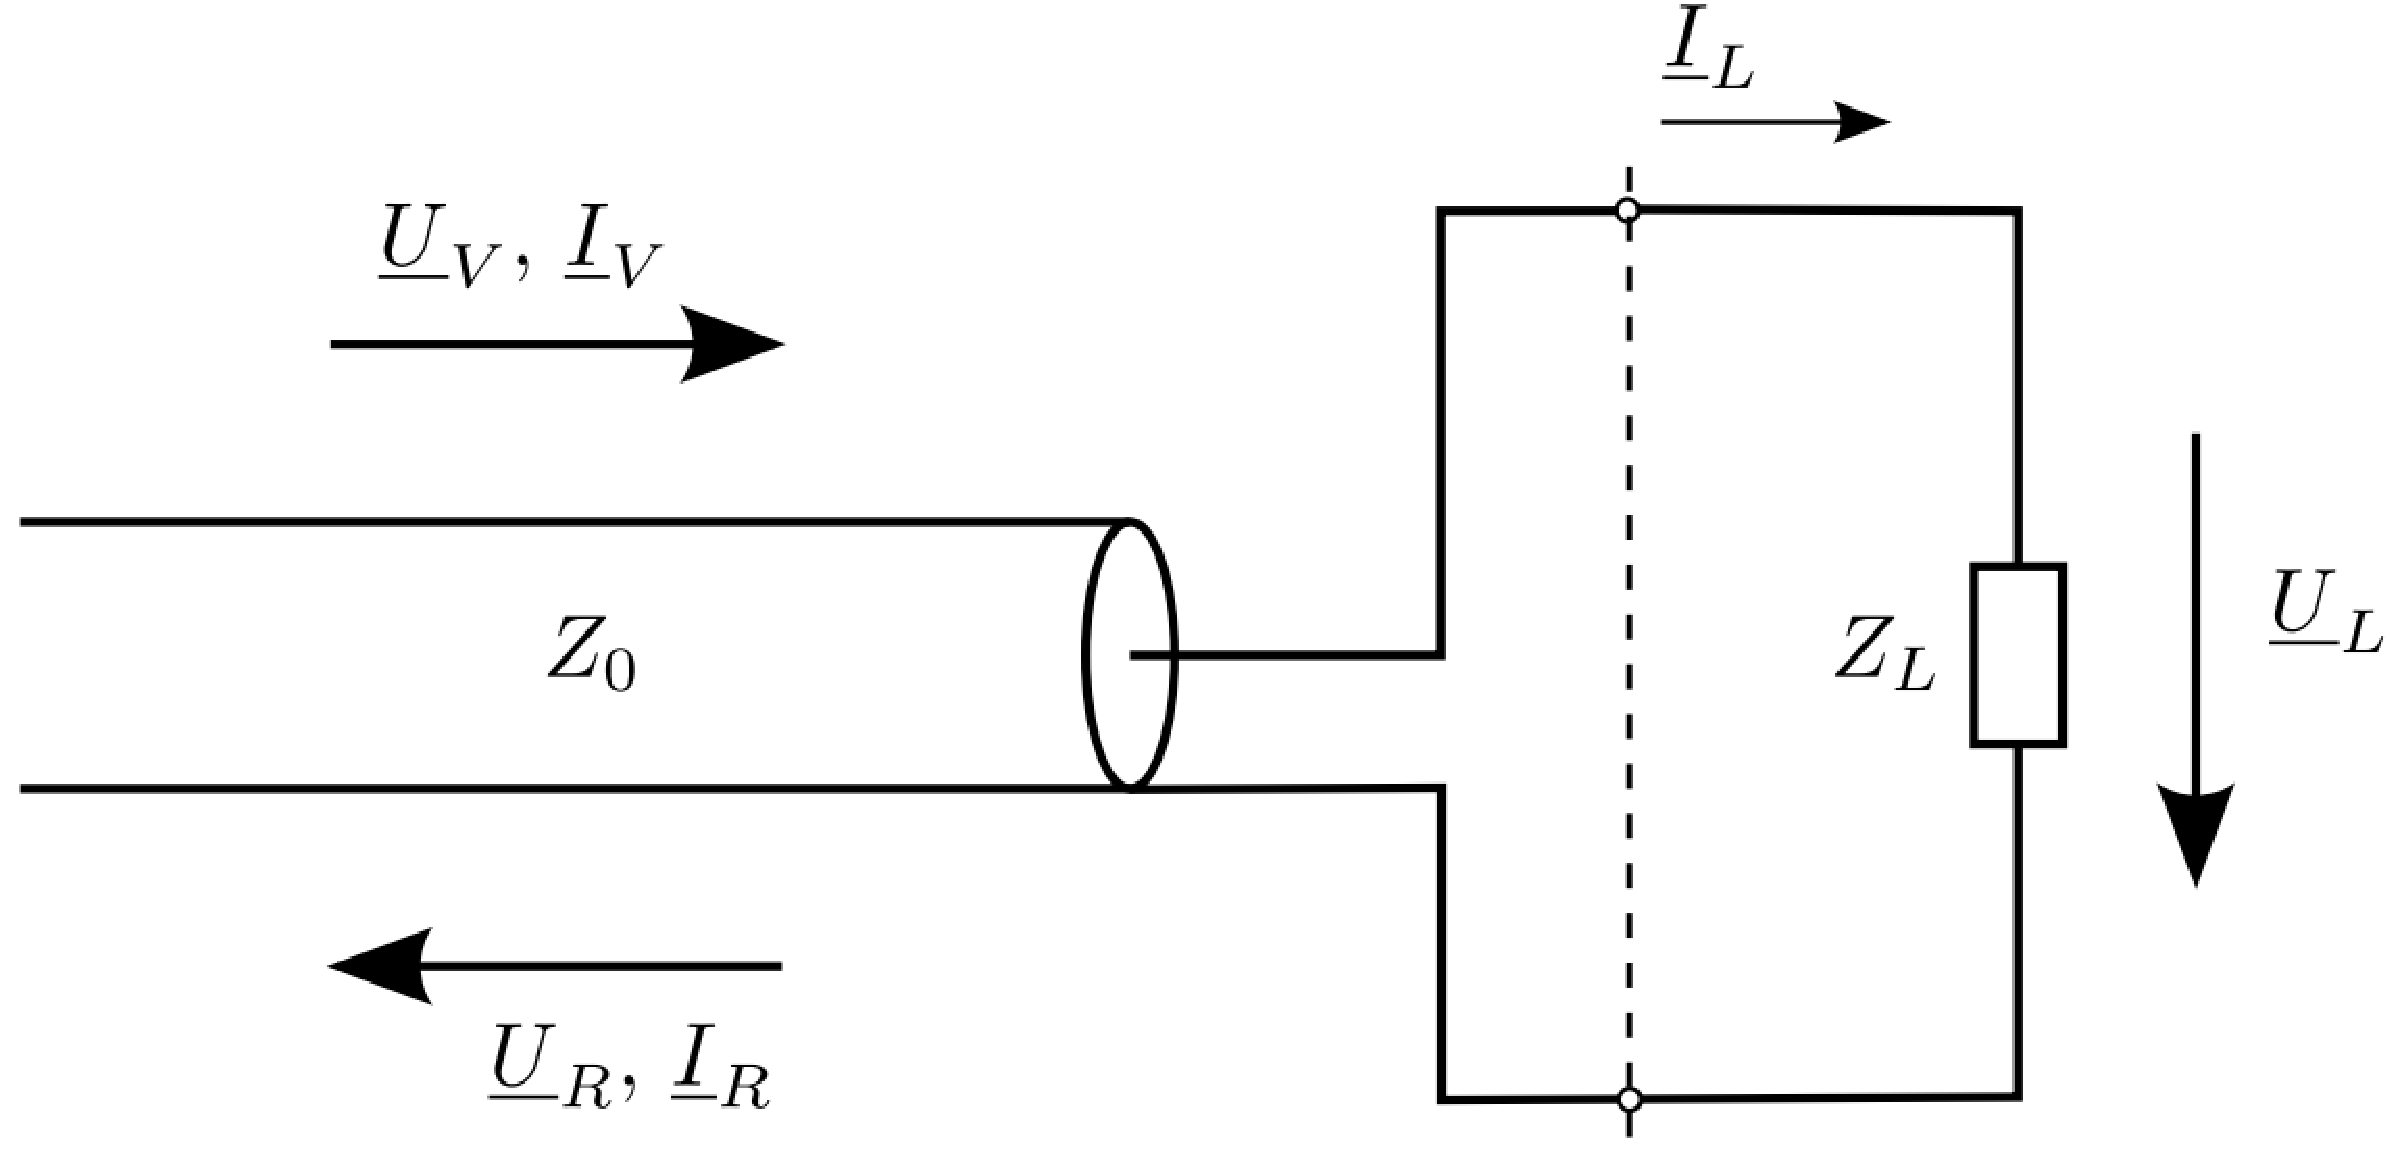
\includegraphics[width=10cm]{content/bilder/ReflexionenLeitungLastimpedanz.pdf}%
	\caption{Signalreflexion an einer Lastimpedanz \cite{Tekom}}
	\label{LeitungMit_ZL}
\end{figure}
%%%%%%%%%%%%%%%%%%%%%%%%%%%%%%%%%%%%%%%%%%%%%%%%%%%%%%%%%%%%%%%%%%%


Die Spannung $\underline{U}_L$ über der Last ergibt sich aus der Summe der vorwärts und der rückwärts laufenden Spannugswellen, wie  in (\ref{eq:AnpassungULast}) gezeigt. Der in der Last fliessende Strom $\underline{I}_L$ wird aus der vorwärts und der rückwärts laufenden Stromwelle gemäss (\ref{eq:AnpassungILast}) berechnet \cite{Tekom}:
\begin{eqnarray}\label{eq:AnpassungULast}
U_L =U_V +U_R
\end{eqnarray}
\begin{eqnarray}\label{eq:AnpassungILast}
I_L = I_V + I_R
\end{eqnarray}
Durch die Überlagerung des vorwärts und des rückwärts laufenden Signals entsteht eine Überlagerungskurve. Unter bestimmten Voraussetzungen bildet sich hierdurch eine stehende Welle in der Leitung. Diese zeichnet sich durch örtlich gebundene Spannungsmaxima $U_{max}$ und -minima $U_{min}$ aus. Desweiteren entstehen Knotenpunkte, an deren Stelle sich die Wellen gegenseitig aufheben, sowie Wellenbergen mit addierten Wellen. Dadurch kann die Spannung an den Knotenpunkten und Wellenbergen Werte zwischen Null und dem doppelten Wert der Spannung des Quellsignals aufweisen.\\

Für die Quantifizierung der Reflexion haben sich neben dem Reflexionskoeffizient $r$ folgende weitere Begriffe etabliert:\\

Rückflussdämpfung $a$, englisch \textit{Return Loss}:

\begin{eqnarray}\label{eq:Ruckflussdämpfung_a}
a=-20\log\left(\left| \dfrac{U_V}{U_R}\right| \right)=-10\log(|r|^{2})
\end{eqnarray}
Die Rückflussdämpfung $a$ beschreibt als logarithmisches Mass, wie stark das rückwärts laufende Signal gegenüber dem vorwärts laufenden Signal gedämpft wird \cite{Tekom}.\\


Welligkeitsfaktor $s$, englisch \textit{Voltage Standing Wave Ratio} (VSWR):
\begin{eqnarray}\label{eq:Welligkeitsfaktor_s}
s=\dfrac{U_{max}}{U_{min}}=\dfrac{1+|r|}{1-|r|}
\end{eqnarray}
Der Welligkeitsfaktor $s$ aus der Gleichung \ref{eq:Welligkeitsfaktor_s} bezieht sich auf das Verhältnis von Spannungsmaxima zu -minima der stehenden Welle \cite{Tekom}.\\

Informationsübermittlungssysteme mit Quelle, Leitung, Verbindungen und Antenne können als eine Kette von Zweitorschaltungen betrachtet werden. Die Eingangsimpedanz eines Zweitors wird oft als $Z_{ein}$, die Ausgangsimpedanz als $Z_{aus}$ bezeichnet. 
Jedes Zweitor kann wiederum als eine Spannungsquelle mit dem Innenwiderstand $Z_I$ verstanden werden, welche mit dem Lastwiderstand $Z_L$ belastet wird. Bei Verwendung hoher Signalfrequenzen oder kurzer Impulsdauer müssen die frequenzabhängigen Eigenschaften dieser Zweitore bei der Entwicklung der Übertragungskette berücksichtigt werden, da wie im Kapitel XX beschrieben Effekte wie Phasenverschiebung oder Signaldämpfung auftreten. Um eine maximale Leistungsübertragung oder eine reflexionsfreie Übertragung im System zu erreichen, werden Anpassungsnetzwerke eingesetzt. Diese führen entweder zu Leistungs- oder Wellenanpassung. Für eine optimale Leistungsübertragung ist es oft notwendig, dass für die verwendete Siganlfrequenz definierte Anpassungsnetzwerke eingesetzt werden.\\


\textbf{Leistungsanpassung } \\
Für die Übertragung der maximalen Wirkleistung von der Quelle zur Last wird Leistungsanpassung benötigt. Hierbei muss gelten \cite{Tekom}:
\[Z_{ein} = Z_{aus}^*\]
Um dies zu erreichen müssen die Realanteile von $Z_{ein}$ und $Z_{aus}$ identisch und die Imaginäranteile betragsmässig gleich sein. Letzteres bedeutet, dass eine induktive Komponente durch eine gleich grosse kapazitive Komponente kompensiert werden muss oder anders gesagt, die Blindwiderstände von Quelle und Last sich gegenseitig aufheben müssen. Dabei sind die Beträge der Imaginäranteile gleich, jedoch ist das Vorzeichen der Winkel der Phasenlage gekehrt, beziehungsweise der Imaginärteil an der Realteilachse gespiegelt. Die Imaginäranteile sind somit konjugiert komplex.\\

\textbf{Wellenanpassung} \\
Bei der Leistungsanpassung kommt es aufgrund der unterschiedlichen Phasenwinkel der Blindwiderstände zu einer Stossstelle für das zu übertragende Signal, wodurch ein Teil des Signals reflektiert wird. Stehende Wellen sind das Resultat. Um diesen für die Signalübermittlung störende Effekt zu vermeiden, wird Wellenanpassung benötigt. Hierbei muss gelten:
\[Z_{ein} = Z_{aus}\]
Das bedeutet, dass die Real- und Imaginäranteile von Quellen- und Lastwiderstand gleich sind, inklusiv dem Phasenwinkel zwischen Real- und Imaginärteil.\\

Bei rein reellem, identischem Innen- und Lastwiderstand, das heisst wenn $X_I = X_L = 0$ gilt, wird Leistungs- und Wellenanpassung erreicht. Es handelt sich hierbei um einen Spezialfall. Für den allgemein gültigen Fall mit komplexen Widerständen ist stets eine Entscheidung zwischen einer Übertragung mit maximaler Wirkleistung unter Inkaufnahme von Teilreflexionen auf den Leitungen oder einer reflexionsfreien Übertragung mit Leistungseinbusse, sprich zwischen Leistungs- und Wellenanpassung zu treffen. In der Nachrichtentechnik bedient man sich in der Regel der Wellenanpassung, da die bei der Leistungsanpassung entstehenden Reflexionen störender sind als die Übertagungsverluste bei verwendeter Wellenanpassung. Bei Leistungsverstärkern eines Senders spielt jedoch die Leistungsanpassung eine nicht zu vernachlässigende Rolle. \\

Die maximale Wirkleistung in der Last wird in einem Gleichstromkreis bei $R_Q = R_L$ abgegeben. Es besteht Leistungsanpassung, das heisst, die im $R_L$ umgesetzte Leistung ist maximal. Der Wirkungsgrad $\eta$ entspricht $50\%$, da dieselbe Leistung in der Last auch im Innenwiderstand der Quelle $R_Q$ umgesetzt wird. Die Formel (\ref{eq:PmaxLeistungsanpassung}) zeigt die maximale Leistung in der Last. Die Abbildung \ref{fig:LeistungsanpassungU0_RQ_RL} zeigt eine Schaltung, bei der die Bedingung für Leistungsanpassung $R_Q = R_L$ gilt.
\begin{eqnarray}\label{eq:PmaxLeistungsanpassung}
P_{Last_{max}}=\dfrac{U_{0}^2}{4R_Q} | R_Q=R_L
\end{eqnarray}

\begin{figure}[!ht]
	\begin{center}
	\begin{tikzpicture}
	\draw[line width=1.5pt](3, 3.5) circle (0.5) node at (3,3.5) {$U_{0}$};%Quelle
	\draw[line width=1.5pt] (3, 5) -- (4.5, 5);%oben kurz

	\draw[line width=1.5pt] (3, 2) -- (3, 3);%von unten zur Quelle
	\draw[line width=1.5pt] (3, 4) -- (3, 5);%von der Quelle nach oben
	\draw[line width=1.5pt](4.5, 4.75) rectangle (5.5, 5.25) node at (5, 5.5) {$R_Q$};%RQ

	\draw[line width=1.5pt, -*](5.5, 5) -- (7, 5);%oben bis zum Punkt
	\draw[line width=1.5pt, -*](3, 2) -- (7, 2);%unten bis zum Punkt
	
	\draw[line width=1.5pt](7, 5) -- (8.5, 5);%oben 
	\draw[line width=1.5pt](7, 2) -- (8.5, 2);%unten 
	\draw[line width=1.5pt](8.5, 5) -- (8.5, 4);%oben nach unten zu RL
	\draw[line width=1.5pt](8.5, 2) -- (8.5, 3);%unten nach oben zu RL

 	\draw[line width=1.5pt](8.25, 3) rectangle (8.75, 4) node at (9.25, 3.5) {$R_L$} ;%RL
% 	\draw[line width=1.5pt, ->, >=latex](6.5, 3.5) -- (7.5, 3.5) node at (7, 3.8) {$P_a$};

	\end{tikzpicture}
	\end{center}
\caption{Leistungsanpassung mit $R_Q = R_L$}
\label{fig:LeistungsanpassungU0_RQ_RL}
\end{figure}
In der Abbildung \ref{fig:LeistungsanpassungU0_RQ_RL} ist eine Leistungsanpassung gezeigt. 
Der Lastwiderstand $R_{L}$ besitzt denselben Widerstandswert wie der Quellenwiderstand $R_{Q}$. Im $R_{L}$ wird wie in (\ref{eq:PmaxLeistungsanpassung}) gezeigt die Hälfte der Quellenleistung umgesetzt.\\
Bei Wechselgrössen kann ein Transformator für die Leistungsanpassung eingesetzt werden. Ist der Quellenwiderstand $R_Q$ oder der Lastwiderstand $R_L$ reaktiv, das heisst induktiv oder kapazitiv, dann sind die Schaltungen stark frequenzabhängig. So besitzt beispielsweise eine Antenne nur bei einer bestimmten Frequenz eine rein reelle Impedanz $Z_{ant}$. Bei allen andern Frequenzen sind sowohl Real- als auch Imaginärteil vorhanden. Als Folge ist Antennenipedanz $Z_{ant}$ komplex. Eine Möglichkeit für eine Anpassung ist in der Abbildung \ref{AnpassungKomplexerLast} dargestellt. Auch diese Anpassung ist frequenzabhängig und nur für die Entwurfsfrequenz optimal.
%%%%%%%%%%%%%%%%%%%%%%%%%%%%%%%%%%%%%%%%%%%%%%%%%%%%%%%%%%%%%%%%%%%
\begin{figure}[!ht]
	\centering
	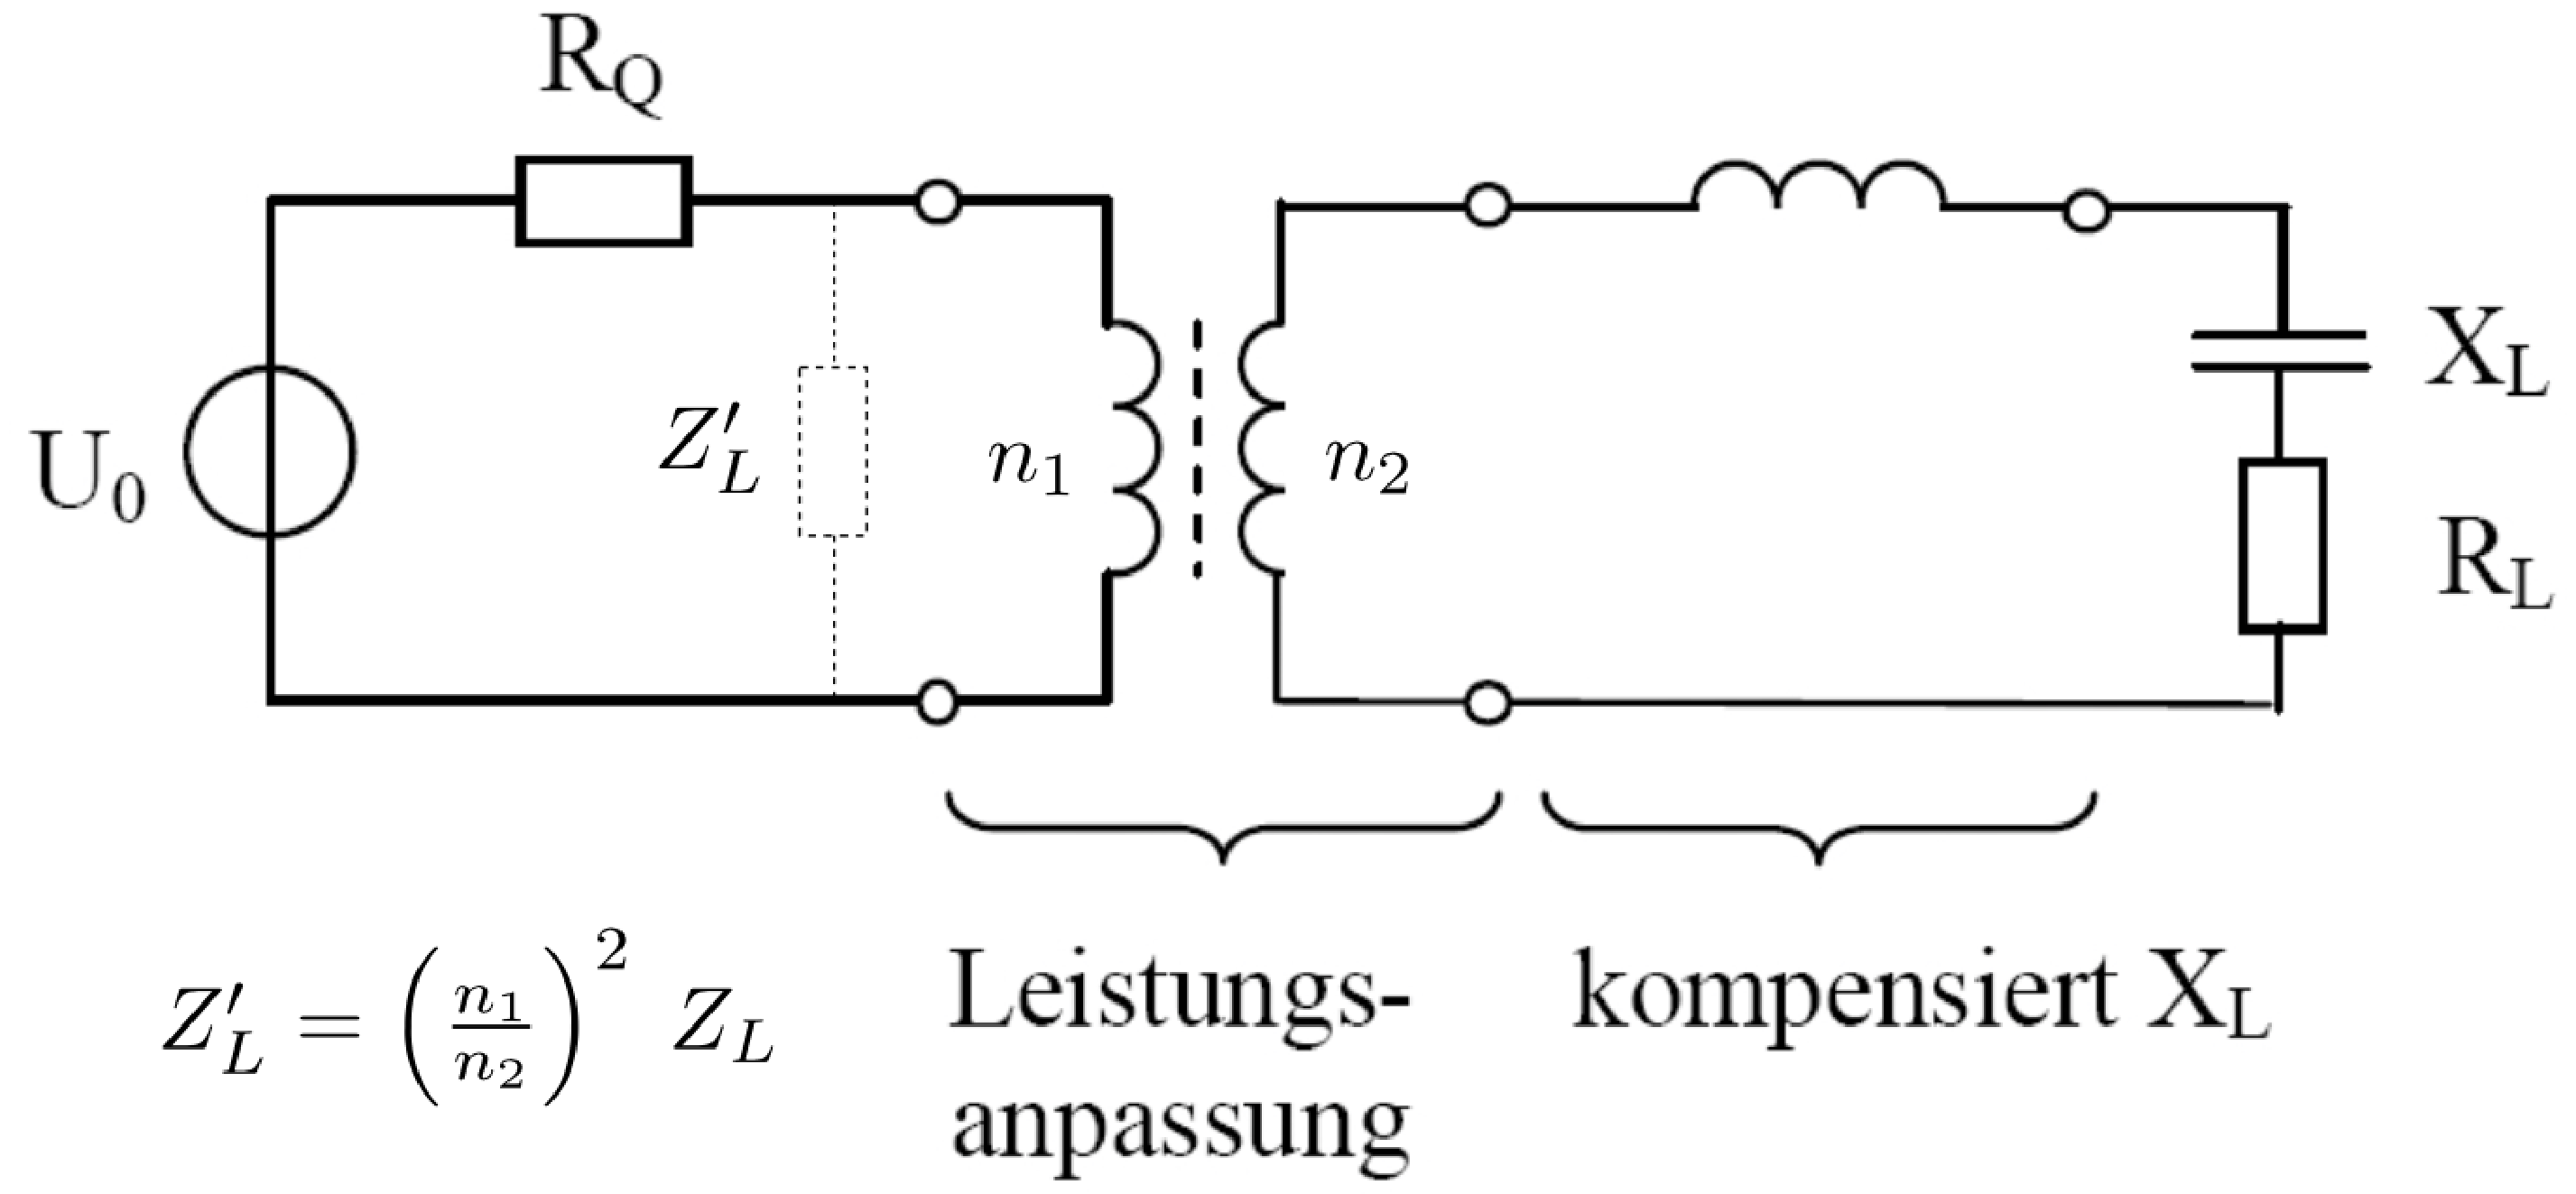
\includegraphics[width=10cm]{content/bilder/AnpassungKomplexerLast.pdf}%
	\caption{Leistungsanpassung für eine komplexe Last mit einem Transformator\cite{Tekom}}
	\label{AnpassungKomplexerLast}
\end{figure}
%%%%%%%%%%%%%%%%%%%%%%%%%%%%%%%%%%%%%%%%%%%%%%%%%%%%%%%%%%%%%%%%%%%
\newpage
\textbf{Entwurf eines Ohm’schen Anpassnetzwerkes} \\
Für die Anpassung einer Generatorimpedanz $R_Q$, welche grösser ist als die Last $R_L$, kann die Schaltung von Abbildung \ref{fig:Leistungsanpassung_RQ_grösser_als_RL} verwendet werden. Die Widerstände R1 und R2 berechnen sich nach folgenden Beziehungen der Gleichungen \ref{eq:R1R2wennRQgrösserRL_R1} und \ref{eq:R1R2wennRQgrösserRL_R2} \cite{Tekom}:
%\begin{equation}
	\begin{align}
		R1 &= \sqrt{R_Q(R_Q-R_L)} \label{eq:R1R2wennRQgrösserRL_R1} \\
		R2 &= \dfrac{R_Q R_L}{R1} \label{eq:R1R2wennRQgrösserRL_R2} \\
		a_{dB} &= 20\log \left( \sqrt{\dfrac{R_Q}{R_L}}+\sqrt{\dfrac{R_Q}{R_L}-1}\right)
	\end{align}
%\end{equation}

\begin{figure}[!ht]
	\begin{center}
	\begin{tikzpicture}
%	\draw[line width=1.5pt](3, 3.5) circle (0.5) node at (3,3.5) {$U_{0}$};%Quelle
%	\draw[line width=1.5pt] (3, 5) -- (4.5, 5);%oben kurz

%	\draw[line width=1.5pt] (3, 2) -- (3, 3);%von unten zur Quelle
	\draw[line width=1.5pt, *-] (1, 5) -- (3, 5);%oben zu R1
	\draw[line width=1.5pt](3, 4.75) rectangle (4, 5.25) node at (3.5, 5.5) {$R1$};%R1

	\draw[line width=1.5pt, *-](5, 5.1) -- (5, 4);%oben nach unten zu RL
	\draw[line width=1.5pt, *-](5, 1.9) -- (5, 3);%unten nach oben zu RL
 	\draw[line width=1.5pt](4.75, 3) rectangle (5.25, 4) node at (5.6, 3.5) {R2};%R2

	\draw[line width=1.5pt, -*](4, 5) -- (7, 5);%oben bis zum Punkt
	\draw[line width=1.5pt, *-*](1, 2) -- (7, 2);%unten bis zum Punkt
	
	\draw[line width=1.5pt](5, 5) -- (8.5, 5);%oben 
	\draw[line width=1.5pt](7, 2) -- (8.5, 2);%unten 
	\draw[line width=1.5pt](8.5, 5) -- (8.5, 4);%oben nach unten zu RL
	\draw[line width=1.5pt](8.5, 2) -- (8.5, 3);%unten nach oben zu RL

 	\draw[line width=1.5pt](8.25, 3) rectangle (8.75, 4) node at (9.25, 3.5) {$R_L$} ;%RL
 	\draw[line width=1.5pt, ->, >=latex](0, 3.5) -- (1.5, 3.5) node at (0.75, 4) {$Z_{ein}=R_Q$};

	\draw[line width=1.5pt,style=dashed](2,1.5) rectangle (6, 6);
	\end{tikzpicture}
	\end{center}
\caption{Anpassung für $R_Q > R_L$}
\label{fig:Leistungsanpassung_RQ_grösser_als_RL}
\end{figure}

Gilt es, eine hochohmige Last $R_L$ an eine Quelle mit einem $R_Q$ der kleiner ist als $R_L$ anzupassen, so kann die Schaltung von Abbildung \ref{fig:LeistungsanpassungU0_RQkleiner_als_RL} und die mathematischen Beziehungen aus \ref{eq:R1R2wennRLgrösserRQ_R1} sowie \ref{eq:R1R2wennRLgrösserRQ_R2} verwendet werden \cite{Tekom}:

\begin{align}
R1 &= \sqrt{R_L(R_L-R_Q)} \label{eq:R1R2wennRLgrösserRQ_R1}\\
R2 &= \dfrac{R_Q R_L}{R1} \label{eq:R1R2wennRLgrösserRQ_R2}\\
a_{dB} &= 20\log \left( \sqrt{\dfrac{R_L}{R_Q}}+\sqrt{\dfrac{R_L}{R_Q}-1}\right)
\end{align}
\begin{figure}[!ht]
	\begin{center}
	\begin{tikzpicture}

	\draw[line width=1.5pt, *-] (1, 5) -- (4, 5);%oben zu R1
	\draw[line width=1.5pt](4, 4.75) rectangle (5, 5.25) node at (4.5, 5.5) {$R1$};%R1

	\draw[line width=1.5pt, *-](3.5, 5.1) -- (3.5, 4);%oben nach unten zu RL
	\draw[line width=1.5pt, *-](3.5, 1.9) -- (3.5, 3);%unten nach oben zu RL
 	\draw[line width=1.5pt](3.25, 3) rectangle (3.75, 4) node at (4, 3.5) {R2};%R2

	\draw[line width=1.5pt, -*](5, 5) -- (7, 5);%oben bis zum Punkt
	\draw[line width=1.5pt, *-*](1, 2) -- (7, 2);%unten bis zum Punkt
	
	\draw[line width=1.5pt](7, 5) -- (8.5, 5);%oben von R1 zum Punkt 
	\draw[line width=1.5pt](7, 2) -- (8.5, 2);%unten 
	\draw[line width=1.5pt](8.5, 5) -- (8.5, 4);%oben nach unten zu RL
	\draw[line width=1.5pt](8.5, 2) -- (8.5, 3);%unten nach oben zu RL

 	\draw[line width=1.5pt](8.25, 3) rectangle (8.75, 4) node at (9.25, 3.5) {$R_L$} ;%RL
 	\draw[line width=1.5pt, ->, >=latex](0, 3.5) -- (1.5, 3.5) node at (0.75, 4) {$Z_{ein}=R_Q$};

	\draw[line width=1.5pt,style=dashed](2,1.5) rectangle (6, 6);
	\end{tikzpicture}
	\end{center}
\caption{Anpassung für $R_Q < R_L$}
\label{fig:LeistungsanpassungU0_RQkleiner_als_RL}
\end{figure}
\newpage
\textbf{Entwurf eines verlustfreien L-Netzwerkes}\\
Ein einfaches, verlustfreies Anpassnetzwerk besteht aus zwei Reaktanzen. Der Entwurfsansatz besteht darin, dass eine Reaktanz $X_{p}$ parallel zum grösseren Widerstand, in Abbildung \ref{fig:verlustfreieAnpassung} wäre dies der Quellenwiderstand $R_{Q}$, geschaltet wird. In diesem Fall kann die Impedanz $Z_{links}$ von der Trennlinie als Parallelschaltung von $R_Q$ und $X_P$ betrachtet werden. \\
Die Impedanz $Z_{links}$ ist definiert als:
\begin{equation}
Z_{Links}= R_{Links}+jX{Links}=\dfrac{R_QX_P^2+jR_Q^2X_P}{R_Q^2+X_P^2}
\end{equation}
$X_P$ kann nun so gewählt werden, dass der Realteil von $Z_{Links}$ dem Lastwiderstand $R_L$ entspricht. \\
\begin{equation}
R_{Links}= R_L
\end{equation}
Als nächstes gilt es, die so eingeführte imaginäre Grösse $X_{Links}$ auf der rechten Seite der 
Trennlinie zu kompensieren, indem die Seriereaktanz $X_{S}$ entsprechend gewählt wird: 
\begin{equation}
X_{Links}= -X_S
\end{equation}
Nun können die Werte für die Induktivität $L$ und Kapazität $C$ für die gewünschte Frequenz berechnet werden. Je nach dem, ob $X_P$ induktiv oder kapazitiv ist, wird $X_S$ gewählt. Durch Umstellen der folgenden Formeln (\ref{eq:XL}) und (\ref{eq:XC}) kann eine Induktivität L oder eine Kapazität C bestimmt werden.
\begin{align}
jX_{L}= j\omega L \label{eq:XL} \\ jX_C=\dfrac{-j}{\omega C} \label{eq:XC}
\end{align} 
%%%%%%%%%%%%%%%%%%%%%%%%%%%%%%%%%%%%%%%%%%%%%%%%%%%%%%%%%%%%%%%%%%%
\begin{figure}[!ht]
	\begin{center}
	\begin{tikzpicture}
	\draw[line width=1.5pt](1, 3) circle (0.5) node at (1,3){$U_0$};
	\draw[line width=1.5pt](1, 3.5) -- (1, 4.5);%quelle nach oben
	\draw[line width=1.5pt](1, 2.5) -- (1, 1.5);%Queelle nach unten
	\draw[line width=1.5pt](1, 4.5) -- (3, 4.5);
	\draw[line width=1.5pt](1, 1.5) -- (10, 1.5);
	\draw[line width=1.5pt](3, 4.75) rectangle (4, 4.25) node at (3.5, 5) {$R_Q$};
	\draw[line width=1.5pt,-*](6, 3.5) -- (6, 4.6);
	\draw[line width=1.5pt,-*](6, 2.5) -- (6, 1.4);
	\draw[line width=1.5pt](5.75, 2.5) rectangle (6.25, 3.5) node at (5.25, 3) {$X_P$};
	\draw[line width=1.5pt, style=dashed](7, 1) -- (7, 5.5) node at (6, 1) {$X_{Links}$};%gestrichelt
	\draw[line width=1.5pt, ->, >=latex](5.25, 1) -- (4, 1);
	\draw[line width=1.5pt](4, 4.5) -- (8, 4.5);%Rq zu XS
	\draw[line width=1.5pt](9, 4.5) -- (10, 4.5);
	\draw[line width=1.5pt](8, 4.75) rectangle (9, 4.25) node at (8.5, 5) {$X_S$};
	\draw[line width=1.5pt](10, 3.5) -- (10, 4.5);
	\draw[line width=1.5pt](10, 2.5) -- (10, 1.5);
	\draw[line width=1.5pt](9.75, 2.5) rectangle (10.25, 3.5) node at (9.25, 3) {$R_L$};
	\end{tikzpicture}
	\end{center}
\caption{Verlustfreie Anpassung}
\label{fig:verlustfreieAnpassung}
\end{figure}
%%%%%%%%%%%%%%%%%%%%%%%%%%%%%%%%%%%%%%%%%%%%%%%%%%%%%%%%%%%%%%%%%%% Wenn ich Zeit habe
%\section{Impedanztransformation einer Leitung}
%\todo{Dieses Kapitel ist fakultativ}
%Phasendrehung auf einer Leitung\\
%$\lambda/4$ Leitung\\
%$\lambda$ Leitung\\
%beliebig lange Leitung\\
%Beispiel im Smith Diagramm mit normierten Werten zeigen
%\section{Anpassung des Antennensystems}
%\todo{beschreiben}
%Welche Möglichkeinten\\
%Leistungsanpssung\\
%Wellenanpassung\\
%Beides, indem der Imaginär Teil verschwindet.\\
%Was steht im Fokus? Die Anpassung ist Richtungsabhängig
%Ein möglichst optimales Empfangensverhalten steht im Vordergurnd
%%%%%%%%%%%%%%%%%%%%%%%%%%%%%%%%%%%%%%%%%%%%%%%%%%%%%%%%%%%%%%%%%%%%%%%%%%%%%%%%%%%%%%%%%%%%%%%%%%%%%%%%%%%%%%%%%%%%
\newpage
\section{Speisung}\label{sec:Speisung}

Unter der Speisung einer Antenne verstanden man die Signalzuführung. Damit eine Antenne strahlt, muss diese mit einer elektromagnetischen Welle angeregt werden. Daraus resultiert eine Strom- und Spannungsverteilung an der Oberfäche der Antenne, diese ist für das Abstrahlverhalten verantwortlich. 
\begin{itemize}
\item 	Leistungsanpassung
\item 	Singalanpassung
\end{itemize}
Leistungsanpassung wird benötigt, wenn der Leistungsfluss möglichst unbeeinträchtigt sein soll. Es muss gelten:
\[Z_{ein}=Z_{aus}*\]
Das bedeutet, dass die Realanteile von $Z_{ein}$ und $Z_{aus}$ gleich sind, jedoch der Imaginärteil von $Z_{aus}$ muss den konjugiert komplexen Wert des $Z_{ein}$ aufweisen. Mit anderen Worten, der Imaginärteil von $Z_{aus}$ hat ein umgekehrtes Vorzeichen als $Z_{ein}$. Leistungsanpassung kommt bei Leistungsendstufen oder allgemein dort zur Anwendung, wo es besonders wichtig ist, dass möglichst viel der erzeugten Leistung von der Last aufgenommen wird. Bei der Leistungsanpassung werden 50\% der erzeugten Leistung in der Quelle und 50\% in der Last umgesetzt.
Wellenanpassung wird angewendet, wenn möglichst keine Reflexionen auf der Leitung entstehen sollen. Es muss gelten:
\[Z_{ein}=Z_{aus}\]
Die Signalanpassung ist dann gewünscht, wenn die Qualität des Signals Vorrang hat und keinerlei Reflexionen erwünscht sind. In diesem Fall ist das Stehwellenverhältnis gleich 1.
Um die gewünschte Anpassung zu erreichen kommen Anpassnetzwerke zum Einsatz. Diese sind meist passive Netzwerke mit Induktivitäten L, Kapazitäten C und Widerständen R.\\
Ein Beispiel für Anpassung.\\
Eine Quelle mit einem Ausgangswiderstand von 50 Ohm reell wird an eine 50 Ohm Leitung angeschlossen. Am Ende der 50 Ohm Leitung wird ein Anpassungsnetzwerk benötigt. Damit wird die Leitung und die Antenne aufeinander abgestimmt. Das Anpassnetzwerk passt die komplexe Antennenimpedanz auf $50\Omega$ reell und $+j0\Omega$ an. In diesem Beispiel wird sowohl Wellen- als auch Leistungsanpassung erfüllt.\\

%%%%%%%%%%%%%%%%%%%%%%

\begin{figure}[!ht]
	\begin{center}
	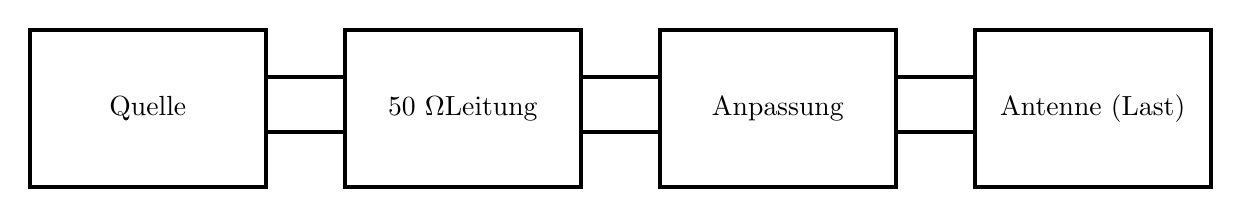
\begin{tikzpicture}
	\draw[line width=1.5pt](0, 0) rectangle (3, 2) node at (1.5, 1) {Quelle};
	\draw[line width=1.5pt](3, 1.4) -- (4, 1.4);
	\draw[line width=1.5pt](3, 0.7) -- (4, 0.7);
	\draw[line width=1.5pt](4, 0) rectangle (7, 2) node at (5.5, 1) {50 $\Omega$Leitung};
	\draw[line width=1.5pt](7, 1.4) -- (8, 1.4);
	\draw[line width=1.5pt](7, 0.7) -- (8, 0.7);
	\draw[line width=1.5pt](8, 0) rectangle (11, 2) node at (9.5, 1) {Anpassung};
	\draw[line width=1.5pt](11, 1.4) -- (12, 1.4);
	\draw[line width=1.5pt](11, 0.7) -- (12, 0.7);
	\draw[line width=1.5pt](12, 0) rectangle (15, 2) node at (13.5, 1) {Antenne (Last)};
	\end{tikzpicture}
	\end{center}
\caption{Blockschaltbild einer Quelle mit Leitung, Anpassung und Antenne}
\label{Anpassung}
\end{figure}

%%%%%%%%%%%%%%%%%%%%%%%%%%%%%%%%%%%%%%%%%%%%%%%%%%%%%%%%%%%%%%%%%%%
%\begin{figure}[!htb]
%	\centering
%	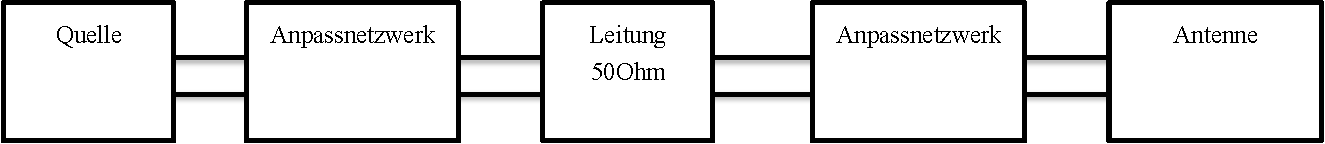
\includegraphics[width=8cm]{content/bilder/Anpassung.pdf}%
%	\caption{Blockschaltbild einer Anpassung von der Quelle zur Antenne}
%	\label{Anpassung}
%\end{figure}
%%%%%%%%%%%%%%%%%%%%%%%%%%%%%%%%%%%%%%%%%%%%%%%%%%%%%%%%%%%%%%%%%%%

\newpage
Wenn eine 50 Ohm Leitung an eine Antenne angeschlossen wird, benötigt man oft ein Anpassnetzwerk zwischen der Leitung und der Antenne. Die Impedanzen der Leitung $Z_L$ und der Antenne $Z_{ant}$ sind nur in seltenen Fällen gleich. Antennen haben einen reellen Strahlungswiderstand $R_{rad}$ und eine Reaktanz $X_{ant}$. Je nach Antennentyp weist $X_{ant}$ einen kapazitiven oder einen induktiven Anteil auf. Die Abbildung \ref{fig:ESBantenne} zeigt das Ersatzschaltbild einer Antenne.
%%%%%%%%%%%%%%%%%%%%%%%%%%%%%%%%%%%%%%%%%%%%%%%%%%%%%%%%%%%%%%%%%%%%
%\begin{figure}[!htb]
%	\centering
%	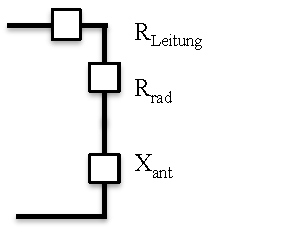
\includegraphics[width=5cm]{content/bilder/ESB_Antenne.pdf}%
%	\caption{Ersatzschaltbild einer Antenne}
%	\label{ESBantenne}
%\end{figure}
%%%%%%%%%%%%%%%%%%%%%%%%%%%%%%%%%%%%%%%%%%%%%%%%%%%%%%%%%%%%%%%%%%%%
\begin{figure}[!ht]
	\begin{center}
	\begin{tikzpicture}
	\draw[line width=1.5pt,*-](12, 5) -- (13.5, 5);%Startz zu Rv
		\draw[line width=1.5pt](14.5, 5) -- (16, 5) ;%Rv zu Rrad
		\draw[line width=1.5pt](16, 5) -- (16, 4.4) ;%Rv zu Rrad
		\draw[line width=1.5pt](14.5, 5) -- (16, 5) ;%
		\draw[line width=1.5pt](13.5, 4.75) rectangle (14.5, 5.25) node at (14, 5.5) {$R_{v}$};
		\draw[line width=1.5pt](15.75, 3.4) rectangle (16.25, 4.4) node at (17, 3.9) {$R_{rad}$};%Rrad
		\draw[line width=1.5pt](16, 3.4) -- (16, 2.8);%Rrad zu Xant
		\draw[line width=1.5pt](15.75, 2.8) -- (16.25, 2.8);%Kondensator oben
		\draw[line width=1.5pt](15.75, 2.6) -- (16.25, 2.6);%Kondensator unten
		\node at (17, 2.7) {$X_{ant}$};
		\draw[line width=1.5pt](16, 2.6) -- (16, 2);
	\draw[line width=1.5pt,-*](16, 2) -- (12, 2);
	\end{tikzpicture}
	\end{center}
\caption{Ersatzschaltbild einer Antenne}
\label{fig:ESBantenne}
\end{figure}

%%%%%%%%%%%%%%%%%%%%%%%%%%%%%%%%%%%%%%%%%%%%%%%%%%%%%%%%%%%%%%%%%%%


%\begin{figure}
%\begin{center}
%\begin{circuitikz}
%\draw (1,1)--(3,1);
%\end{circuitikz}
%\end{center}
%\end{figure}
%%%%%%%%%%%%%
%%%%%%%%%%%%%%%%%%%%%%
%\begin{ circuitikz }[ scale =1.2]
%\begin{tikzpicture}
%\draw(0,0) node[anchor=east]{B} to [short, o-*] (1,0)
%to [R=20<\ohm>, *-*] (1,2)
%%to [R=10<\ohm>, v=$v_x$] (3,2) −− (4,2)
%%to [ cI=$\frac{\siemens}{5} v_x$, *−*] (4,0) −− (3,0)
%%to [R=5<\ohm>, *−*] (3,2)
%(3,0) −− (1,0)
%(1,2) to [short, −o] (0,2) node[anchor=east]{A};
%\end{tikzpicture}
%\end{ circuitikz }
%%%%%%%%%%%%%%%%%%%%%%
Wenn man die Speisung in einem grösseren Zusammenhang betrachtet, dann erkennt man, dass die Speisung mehr als die Berücksichtigung der Impedanzen von der Quelle bis zur Antenne umfasst. Um eine Aussage über die Speisung einer Antenne zu machen, muss mehr als nur die Ausgangsimpedanz der Quelle $Z_{aus}$ und die Eingangsimpedanz der Antenne $Z_{ant}$ bekannt sein. Die Abbildung \ref{AnpassungQuelleAntenne} zeigt wichtige Zusammenhänge der Speisung und des Zusammenhangs von Quelle, Leitungsimpedanz und der Antenne auf. Wie im Kapitel \ref{sec:AnpassungReflexionen} ist die Anpassung der Zuleitung an die Antenne massgebend für den Reflexionskoeffizient $\Gamma$, aus dem wiederum auf die Reflexionsdämpfung |$S_{11}$| geschlossen wird. Der Zusammenhang ist einfach. Je mehr der Reflexionskoeffizient $\Gamma\rightarrow 1$ geht, desto grösser ist der |$S_{11}$| Wert in dB. Dadurch gelangt mehr Leistung in die Antenne, somit kann mehr Energie abgestrahlt werden. Die Abstrahlleistung $P_{rad}$ ist abhängig von $R_{rad}$. Denn $P_{rad}$ ist als $P_{rad}=1/2*I_{ant}^2*R_{rad}$ definiert. Aus der Abstrahleffizienz $\eta_{rad}$ ist ebenfalls zu erkennen, dass die Verluste des Antennensystems klein gegenüber dem Abstrahlwiderstand $R_{rad}$ sein müssen. Dies führt zu einer hohen Abstrahleffizienz $\eta_{rad}$.

\begin{figure}[!ht]
	\begin{center}
	\begin{tikzpicture}
	\draw[line width=1.5pt](3, 3.5) circle (0.5) node at (3,3.5) {Uq};
	\draw[line width=1.5pt] (3, 5) -- (4.5, 5);
	%\draw[line width=1.5pt] (3, 2) -- (7, 2);
	\draw[line width=1.5pt, -*](3, 2) -- (7, 2);
	\draw[line width=1.5pt] (3, 2) -- (3, 3);
	\draw[line width=1.5pt] (3, 4) -- (3, 5);
	\draw[line width=1.5pt](4.5, 4.75) rectangle (5.5, 5.25) node at (5, 5.5) {Rq} node at (5, 4.5) {50 Ohm};
	%\draw[line width=1.5pt] (5.5, 5) -- (7, 5);
	\draw[line width=1.5pt, -*](5.5, 5) -- (7, 5);
	
	\draw[line width=1.5pt](7, 1.5) rectangle (12, 5.5) node at (9.5, 5) {Anpassungsnetzwerk} node at (9.5, 4.5) {Leitung};
	\draw[line width=1.5pt, *-](12, 5) -- (13.5, 5);
	\draw[line width=1.5pt, *-](12, 2) -- (16, 2);
	\draw[line width=1.5pt](13.5, 4.75) rectangle (14.5, 5.25) node at (14, 5.5) {$R_{v}$};
	\draw[line width=1.5pt](14.5, 5) -- (16, 5);
	\draw[line width=1.5pt](16, 5) -- (16, 4.4);
	\draw[line width=1.5pt](15.75, 3.4) rectangle (16.25, 4.4) node at (17, 3.9) {$R_{rad}$};%Rrad
	\draw[line width=1.5pt](16, 3.4) -- (16, 2.8);
	\draw[line width=1.5pt](15.75, 2.8) -- (16.25, 2.8);%Kondensator oben
	\draw[line width=1.5pt](15.75, 2.6) -- (16.25, 2.6);%Kondensator unten
	\node at (17, 2.7) {$X_{ant}$};
	\draw[line width=1.5pt](16, 2.6) -- (16, 2);
	
	\draw[line width=1.5pt, ->, >=latex](6.5, 4) -- (8, 4) node at (8, 3.5) {$P_{ein}$};
	\draw[line width=1.5pt, ->, >=latex](11.5, 4) -- (13, 4) node at (13, 3.5) {$P_{ant}$};
	
	\coordinate (A) at (5, 1);
	\coordinate (B) at (4.8, 0);
	\coordinate (a) at (8, 0.5);
	\draw[line width=1.5pt, cap=round,->](A) .. controls (a) .. (B) node at (5, 0.5) {$\Gamma$};
	\draw [-latex,line width=1.5pt](11.5,1) |-(13,2.5) node at (11.5, 0.5) {$Z_{ant}$};
	
	\node at (17.5, 6.2) {$\eta_{rad}=\dfrac{R_{rad}}{Rv+R_{rad}}$};
	\node at (9.5, 6.2) {$\eta_{overall}=\dfrac{P_{rad}}{P_{ein}}$};
	
	\node at (18, 2.7) {$\varepsilon$};
	\node at (18.5, 2.7) {$\delta$};
	
	\draw[->,line width=0.5pt,decorate, decoration=snake ](18, 4.1) -- (19.5, 4.6);
	\draw[->,line width=0.5pt, decorate, decoration=snake](18, 3.9) -- (19.5, 3.9);
	\draw[->,line width=0.5pt, decorate, decoration=snake](18, 3.7) -- (19.5, 3.1);
	\node at (20, 3.9) {$P_{rad}$};
	\end{tikzpicture}
	\end{center}
\caption{ESB einer Quelle mit Anpassnetzwerk, Leitung und einer Antenne}
\label{AnpassungQuelleAntenne}
\end{figure}











